% !TEX program = xelatex
\documentclass[11pt,a4paper]{article}

% ===== フォント・日本語 =====
\usepackage{fontspec}
\setmainfont{Noto Serif CJK JP}[AutoFakeSlant=0.2]
\setsansfont{Noto Sans CJK JP}
\newfontfamily\jpfont{Noto Serif CJK JP}

% ===== CJK 行分割を有効化（xeCJK 不在環境向け） =====
% XeTeX のプリミティブで CJK 文字間に分割可能点を挿入する
\XeTeXlinebreaklocale "ja"
\XeTeXlinebreakskip = 0pt plus 0.1pt minus 0.01pt
% 和文中の禁則・体裁の微調整
\XeTeXlinebreakpenalty = 0

% 数式境界などで生じる僅かなはみ出しを吸収する
\emergencystretch=3em

% ===== レイアウト =====
\usepackage[a4paper,margin=25mm]{geometry}
\usepackage{parskip}
\linespread{1.15}

% ===== 数式 =====
\usepackage{amsmath,amssymb,mathtools}
\usepackage{bm}

% ===== 図・表・色 =====
\usepackage{graphicx}
\usepackage{xcolor}
\usepackage{booktabs}
\usepackage{array}
\usepackage{tabularx}
\usepackage{tikz}
\usetikzlibrary{arrows.meta,positioning,calc,decorations.pathmorphing,backgrounds}

% ===== ハイパーリンク =====
\usepackage[colorlinks=true,linkcolor=darkblue,urlcolor=darkblue,citecolor=darkblue]{hyperref}

% ===== 色定義 =====
\definecolor{darkblue}{RGB}{20,60,120}
\definecolor{accent}{RGB}{180,60,40}
\definecolor{boxbg}{RGB}{244,247,252}
\definecolor{boxrule}{RGB}{120,150,200}
\definecolor{warnbg}{RGB}{253,247,238}
\definecolor{warnrule}{RGB}{200,140,60}

% ===== ボックス環境 =====
\usepackage[most]{tcolorbox}
\newtcolorbox{keybox}[1][]{
  colback=boxbg, colframe=boxrule, boxrule=0.6pt, arc=2pt,
  left=8pt,right=8pt,top=6pt,bottom=6pt, #1}
\newtcolorbox{warnbox}[1][]{
  colback=warnbg, colframe=warnrule, boxrule=0.6pt, arc=2pt,
  left=8pt,right=8pt,top=6pt,bottom=6pt, #1}

% ===== 見出し体裁 =====
\usepackage{titlesec}
\titleformat{\section}{\Large\bfseries\color{darkblue}}{\thesection}{0.6em}{}
\titleformat{\subsection}{\large\bfseries\color{darkblue}}{\thesubsection}{0.6em}{}
\titleformat{\subsubsection}{\normalsize\bfseries\color{accent}}{\thesubsubsection}{0.6em}{}
\titlespacing*{\section}{0pt}{2.2ex plus 1ex minus .2ex}{1.2ex plus .2ex}

% ===== 便利マクロ =====
\newcommand{\es}{\bm{e}_{s}}
\newcommand{\esp}{\bm{e}_{s\perp}}
\newcommand{\rv}{\bm{r}}
\newcommand{\Fv}{\bm{F}}
\newcommand{\Mab}{\bm{M}_{ab}}
\newcommand{\Maa}{\bm{M}_{aa}}
\newcommand{\gamz}{\gamma_{0}}
\newcommand{\dd}{\mathrm{d}}
\newcommand{\Dopt}{\Delta_{\mathrm{opt}}}

% 長いコードパスを任意位置で折り返せるようにするマクロ
\usepackage{seqsplit}
\newcommand{\cp}[1]{{\ttfamily\expandafter\seqsplit\expandafter{\detokenize{#1}}}}

\begin{document}

% ===================== 表紙 =====================
\begin{titlepage}
\centering
\vspace*{2.5cm}
{\color{darkblue}\rule{\linewidth}{1.2pt}}\\[6pt]
{\Huge\bfseries 1次元スライダーモデル}\\[10pt]
{\LARGE 物理・数学・数値手法の網羅的解説}\\[8pt]
{\large（exp01 〜 exp05 実装の理論ガイド）}\\[6pt]
{\color{darkblue}\rule{\linewidth}{1.2pt}}\\[1.5cm]

{\large 繊毛簡略化モデルにおける}\\[4pt]
{\large 流体力学的相互作用と周期平均正味流量 $Q$}\\[2cm]

\begin{minipage}{0.85\linewidth}
\small
本文書は、修士論文第4章の 1D スライダーモデルを Python で段階的に再実装した
プロジェクト（\texttt{cilia\_simulation}）について、exp05 までに実装した
物理モデル・支配方程式・数値手法・コード対応を、初学者でも追えるように
体系的に解説するものである。
\end{minipage}

\vfill
{\large 実装基準時点：2026年6月（exp05 完了時点）}\\[4pt]
\end{titlepage}

\tableofcontents
\newpage

% ===================== 1 はじめに =====================
\section{はじめに ── 何を計算しているのか}

\subsection{物理的な舞台設定}

生物の表面を覆う\textbf{繊毛（cilia）}は、規則的に打つことで周囲の流体を一方向に
輸送する。多数の繊毛が少しずつ位相をずらして打つと「メタクロナル波」が生じ、
正味の流れが効率よく作られる。この現象の本質を、最小限の要素で取り出したのが
\textbf{1次元スライダーモデル}である。

このモデルでは、繊毛1本を「傾いた直線レール上を往復運動する小さなビーズ」に
置き換える。ビーズ（スライダー）には外部から周期的な駆動力が加わり、ばねで
中心に引き戻されながら、低レイノルズ数の粘性流体の中を振動する。
ビーズが動くと流体を押し、流体を介して隣のビーズと相互作用する。

\begin{keybox}
\textbf{最終目標}：流体力学的相互作用によって生じる
\emph{周期平均正味流量} $Q$ と、それを最大化する
\emph{最適位相差} $\Dopt$ が、スライダー間距離 $l$ にどう依存するかを
数値的に再現すること（論文第4章）。
\end{keybox}

\subsection{なぜ「段階的」に実装するのか}

複雑なモデルをいきなり書くとバグの切り分けが難しい。そこで
「単体 $\to$ 2体（壁なし）$\to$ パラメータ掃引 $\to$ 壁あり」と
物理的要素を一つずつ増やし、各段階で理論解や対称性による検証を行う。

\begin{table}[h]
\centering\small
\begin{tabularx}{\linewidth}{l l X l}
\toprule
段階 & スクリプト & 内容 & 状態 \\
\midrule
exp01 & \texttt{exp01\_single\_slider.py} & 単一スライダー、壁なし & 完了 \\
exp02 & \texttt{exp02\_two\_sliders\_nowall.py} & 2本、Oseen 相互作用 & 完了 \\
exp03 & \texttt{exp03\_sweep\_delta\_l.py} & $\Delta\times l$ 掃引、$Q(\Delta,l)$ 解析 & 完了 \\
exp04 & \texttt{exp04\_two\_sliders\_wall.py} & 壁あり Blakelet（単点検証） & 完了 \\
exp05 & \texttt{exp05\_sweep\_delta\_l\_wall.py} & 壁あり Blakelet の $\Delta\times l$ 掃引 & 完了 \\
exp06 & \texttt{exp06\_sweep\_delta\_theta.py} & $\Delta\times\theta$ 掃引（$l$ 固定） & 未実装 \\
\bottomrule
\end{tabularx}
\end{table}

\subsection{段階ごとの流体力学（最重要の整理）}

このプロジェクトでは「流体力学」が2か所に登場する。すなわち
\textbf{(1) 力$\to$速度を結ぶ移動度}と、\textbf{(2) 流量 $q_x$ の指標定義}である。
段階が進むにつれて(1)が変わるので、結果を読むときは段階を必ず意識する。

\begin{table}[h]
\centering\small
\begin{tabularx}{\linewidth}{l X X}
\toprule
段階 & 移動度（力$\to$速度） & 流量 $q_x$ の指標 \\
\midrule
exp01〜03 & Oseen／Stokeslet（\emph{壁なし}） & 式(2.61)（壁 $z=0$ 遠方近似） \\
exp04〜05 & \textbf{Blakelet（壁 $z=0$ あり）} & 式(2.61)(4.65)（移動度と整合） \\
\bottomrule
\end{tabularx}
\end{table}

\begin{keybox}
\textbf{exp03 まで}：移動度は壁なし Oseen なのに、流量指標は壁前提の式(2.61) を
借りている。両者が不整合なので、exp03 の結果は\textbf{定性的トレンドと数値
パイプラインの検証}として位置づける。\\[4pt]
\textbf{exp04 以降}：移動度を\textbf{Blakelet（壁 $z=0$ で滑りなし）}に置き換え、
流量指標と物理的に整合させた。これにより論文最終形に対応する。論文 Fig との
\textbf{定量比較は exp05 の fine 掃引}（\texttt{-{}-mode fine}）で評価する。
\end{keybox}

なお、本資料の理論章（第\ref{sec:theory}章）は論文の遠距離漸近解析に対応し、
移動度として Blakelet を用いる。したがって理論は exp04〜05（Blakelet 実装）と
直接対応し、exp03（Oseen）とは定性的トレンドのレベルで対応する。

% ===================== 2 幾何 =====================
\section{幾何・座標系・無次元化}

\subsection{座標軸の役割}

3つの軸はそれぞれ明確な物理的意味を持つ。

\begin{itemize}
\item $x$：\textbf{流れ方向}。正味流量 $Q$ を評価する向き。
\item $y$：流れに垂直。本問題は $y=0$ 平面内の実質2D問題。
\item $z$：\textbf{壁の法線方向}。壁は $z=0$ に存在する（exp03 までは
移動度に未反映、exp04 以降は Blakelet で反映）。
\end{itemize}

\subsection{スライダーの幾何（図解）}

各スライダーは傾き角 $\phi$ の直線レール上を、スカラー座標 $s_i(t)$ で運動する。

\begin{figure}[h]
\centering
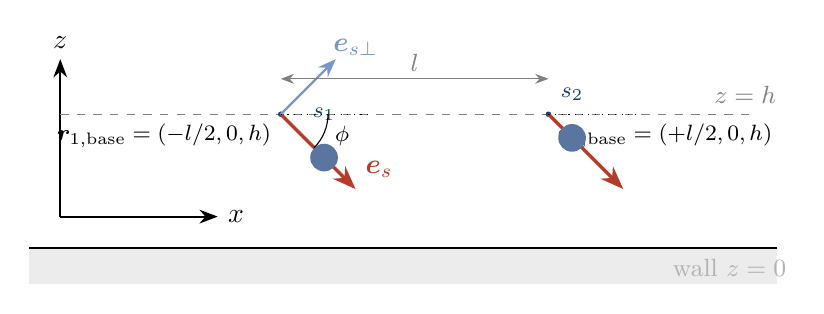
\begin{tikzpicture}[scale=1.0,>=Stealth]
  % wall
  \fill[gray!15] (-1,-0.45) rectangle (8.5,0);
  \draw[thick] (-1,0)--(8.5,0);
  \node[gray!60] at (7.9,-0.25){\small wall $z=0$};
  % axes
  \draw[->,thick] (-0.6,0.4)--(1.4,0.4) node[right]{$x$};
  \draw[->,thick] (-0.6,0.4)--(-0.6,2.4) node[above]{$z$};
  % base height line
  \draw[dashed,gray] (-0.6,1.7)--(8.2,1.7);
  \node[gray] at (8.1,1.95){\small $z=h$};

  % --- slider 1 ---
  \coordinate (b1) at (2.2,1.7);
  \fill[darkblue] (b1) circle (1pt);
  \node[below left] at (b1) {\footnotesize $\bm{r}_{1,\mathrm{base}}=(-l/2,0,h)$};
  % rail direction e_s = (cos phi,0,-sin phi), phi=45 -> down-right
  \draw[->,accent,very thick] (b1)--($(b1)+(0.95,-0.95)$);
  \node[accent] at ($(b1)+(1.25,-0.7)$){$\es$};
  % bead on rail
  \fill[darkblue!70] ($(b1)+(0.55,-0.55)$) circle (5pt);
  \node[darkblue] at ($(b1)+(0.55,-0.55)+(0.0,0.55)$){\footnotesize $s_1$};
  % perp
  \draw[->,boxrule,thick] (b1)--($(b1)+(0.7,0.7)$);
  \node[boxrule] at ($(b1)+(0.95,0.85)$){$\esp$};
  % angle
  \draw (b1)++(0.6,0) arc (0:-45:0.6);
  \node at ($(b1)+(0.78,-0.28)$){\footnotesize $\phi$};
  \draw[dotted] (b1)--($(b1)+(1.1,0)$);

  % --- slider 2 ---
  \coordinate (b2) at (5.6,1.7);
  \fill[darkblue] (b2) circle (1pt);
  \node[below right] at (b2) {\footnotesize $\bm{r}_{2,\mathrm{base}}=(+l/2,0,h)$};
  \draw[->,accent,very thick] (b2)--($(b2)+(0.95,-0.95)$);
  \fill[darkblue!70] ($(b2)+(0.30,-0.30)$) circle (5pt);
  \node[darkblue] at ($(b2)+(0.30,-0.30)+(0.0,0.55)$){\footnotesize $s_2$};
  \draw[dotted] (b2)--($(b2)+(1.1,0)$);

  % distance l
  \draw[<->,gray] (2.2,2.15)--(5.6,2.15);
  \node[gray] at (3.9,2.35){\small $l$};
\end{tikzpicture}
\caption{2本スライダーの配置。各ビーズは傾き角 $\phi$ の直線レール（$\es$ 方向）
上をスカラー $s_i$ で動く。中心間距離は $l$、基準高さは $h$。$\phi>0$ では
レールは壁側（$z$ 負方向）へ傾く。}
\end{figure}

\textbf{直線方向の単位ベクトル}（\texttt{core/slider.py}）：
\begin{equation}
\es=(\cos\phi,\ 0,\ -\sin\phi)
\end{equation}
$\phi>0$ のとき $z$ 成分が負となり、ビーズは壁側へ傾く。

\textbf{直線に垂直な単位ベクトル}（\texttt{core/solver.py}）：
\begin{equation}
\esp=(\sin\phi,\ 0,\ \cos\phi),\qquad \es\cdot\esp=0
\end{equation}

\subsection{2体配置}

論文 式(4.1)(4.2) に合わせ、基準位置と瞬時位置は
\begin{align}
\rv_{1,\mathrm{base}}&=\Big(-\tfrac{l}{2},0,h\Big), &
\rv_{2,\mathrm{base}}&=\Big(+\tfrac{l}{2},0,h\Big),\\[4pt]
\rv_1(t)&=\rv_{1,\mathrm{base}}+s_1(t)\,\es, &
\rv_2(t)&=\rv_{2,\mathrm{base}}+s_2(t)\,\es.
\end{align}
ここで $l>0$ は中心間距離、$h>0$ は壁からの基準高さである。

\subsection{無次元化：コードと論文を切り離して理解する}\label{sec:nondim}

無次元化については、\textbf{2つの異なる体系}を混同しないことが重要である。
ひとつは\emph{このコードが実際に採用している}無次元化、もうひとつは\emph{論文
2.4節}が定義する無次元化で、両者は別モデルに属する。まずコード側を確定し、
次に論文側を参考として示し、最後に両者の関係を整理する。

\subsubsection{(A) このコードの無次元化}

\begin{keybox}
\textbf{コードは次元変換を一切しない}。\texttt{config/default\_params.py} の数値は
「すでに無次元化済みの量」として、そのまま運動方程式に代入される。SI単位からの
換算や、代表量で割る前処理（\texttt{nondimensionalize()} のような関数）は存在しない。
参照スケールは\textbf{デフォルト値（多くが $1$）として式の中に埋め込まれている}。
\end{keybox}

つまり、このコードでは「何かを何かで割って無次元にする」という操作は\emph{行われず}、
代わりに\textbf{各基準量を $1$ に選ぶ}ことでスケールを固定している。具体的には、
次の暗黙の参照単位が採られている。

\begin{table}[h]
\centering\small
\begin{tabularx}{\linewidth}{l l X}
\toprule
種類 & 基準量（$=1$ に固定） & 意味 \\
\midrule
長さ & $h=1$ & $l,s,a$ も同じ長さ単位（$l=2,a=0.05$ など） \\
力 & $F_0=1$ & 能動力振幅を力の単位に取る \\
粘性 & $\mu=1$ & 粘性係数を単位に取る \\
剛性 & $k=1$ & 復元力 $-ks$ のばね定数 \\
時間 & $\omega=2\pi$ & 周期 $T=2\pi/\omega=1$（1打周期 $=$ 時間1） \\
角度 & $\phi,\Delta$ [rad] & もともと無次元 \\
\bottomrule
\end{tabularx}
\end{table}

この単位系のもとで、コード内の式はそのまま無次元式として閉じている。主要なものを
無次元グループの観点で並べると：
\begin{align}
\text{移動度：}&\quad \gamz=\frac{1}{6\pi\mu a},\\
\text{単体 ODE：}&\quad \frac{\dd s}{\dd t}=\gamz\big(F_0\cos\omega t-ks\big),\\
\text{2体駆動：}&\quad f_{\mathrm{active},1}=F_0\cos(\omega t+\Delta),\ \
f_{\mathrm{active},2}=F_0\cos(\omega t),\\
\text{流量（単体）：}&\quad q_x=\frac{h}{\pi\mu}F_x,\quad F_x=f_{\mathrm{total}}\cos\phi,\\
\text{流量（2体）：}&\quad q_x=\frac{1}{\pi\mu}\big[z_1F_{x,1}+z_2F_{x,2}\big],\quad
z_i=h-s_i\sin\phi,\\
\text{周期平均：}&\quad Q=\frac{1}{T}\int q_x\,\dd t\quad(\text{定常窓}=\text{最後の1周期}).
\end{align}

\begin{table}[h]
\centering\small
\begin{tabularx}{\linewidth}{c X c X}
\toprule
記号 & 意味 & 既定値 & 役割 \\
\midrule
$a$ & ビーズ半径 & 0.05 & 移動度 $\gamz=1/(6\pi\mu a)$。$h$ 単位での相対サイズ \\
$\mu$ & 粘性係数 & 1.0 & 粘性の基準（$=1$） \\
$k$ & ばね定数 & 1.0 & 剛性の基準（$=1$） \\
$F_0$ & 駆動力振幅 & 1.0 & 力の基準（$=1$） \\
$\omega$ & 角振動数 & $2\pi$ & 時間の基準（$T=1$） \\
$\phi$ & 傾き角 & $\pi/4$ & 45$^\circ$。形状パラメータ \\
$h$ & 基準高さ & 1.0 & 長さの基準（$=1$） \\
$l$ & 中心間距離 & 2.0 & exp03 掃引対象（$l\in[1.5,6]$） \\
$\Delta$ & 位相差 & $\pi/2$ & exp03 掃引対象（$[-\pi,\pi)$） \\
$s_1(0),s_2(0)$ & 初期位置 & 0 & \\
\bottomrule
\end{tabularx}
\end{table}

\begin{keybox}
\textbf{真に意味を持つ無次元パラメータ}：基準量 $\mu,k,F_0,h,\omega$ を $1$（と $2\pi$）に
固定したあと、結果に効くのは
\begin{itemize}\setlength{\itemsep}{1pt}
\item $a=0.05$（$h$ に対するビーズの相対サイズ）
\item $\phi$（傾き角）と $l$（$h$ に対する間距離）── exp03 の掃引軸
\item $\Delta$（位相差）
\item 振幅・位相遅れを決める比 $\omega/(k\gamz)$
\end{itemize}
である。$Q$ の自然なスケールは $F_0 h/(\pi\mu)$ で、exp01 の成功判定
（\texttt{check\_Q\_near\_zero} の \texttt{reference\_scale}）にも使われる。
\end{keybox}

\subsubsection{(B) 論文 2.4 節の無次元化（参考：別モデル）}

論文 2.4 節は、第2〜3章の\textbf{トルク駆動ばねビーズモデル}に対して無次元化を
定義している。これは\emph{このスライダーコードとは別のモデル}だが、背景として
押さえておくと論文を読む助けになる。代表量は\textbf{代表長さ $L$（繊毛長）・
代表トルク $\tau_{\max}$・粘性 $\mu$} の3つで（式(2.63)〜(2.67)）：
\begin{gather}
\rv^{\ast}=\frac{\rv}{L},\quad a^{\ast}=\frac{a}{L},\quad
\tau_k^{\ast}=\frac{\tau_k}{\tau_{\max}}\ (|\tau_k^{\ast}|\le1),\quad
q_x^{\ast}=\frac{\mu}{\tau_{\max}}q_x,\\[4pt]
k_s^{\ast}=\frac{k_s L^2}{\tau_{\max}},\quad k_b^{\ast}=\frac{k_b}{\tau_{\max}},\qquad
t^{\ast}=\frac{\tau_{\max}}{\mu L^2}\,t.
\end{gather}

\begin{keybox}
\textbf{時間スケールの出どころ}：過減衰系では「トルク $=$ 抵抗 $\times$ 速度」。
抵抗は $\mu L$、速度は $L/t$ の次元なので $\tau_{\max}\sim\mu L\cdot(L/t)\cdot L
=\mu L^3/t$、すなわち $t\sim\mu L^2/\tau_{\max}$ が自然な時間スケールになる。
\end{keybox}

\subsubsection{(C) 両者の関係と注意}

\begin{warnbox}
\textbf{コードの無次元化は論文2.4節の「適用」ではない}。両者は駆動の種類からして
違う：論文2.4節は\emph{トルク $\tau_{\max}$ 駆動}、スライダーコードは
\emph{力 $F_0$・ばね $k$ 駆動}である。したがって $\tau_{\max}$、$k_s^{\ast}$、
$k_b^{\ast}$、時間スケール $\mu L^2/\tau_{\max}$ は\textbf{コードには現れない}。
とくに論文の流量無次元化 $q_x^{\ast}=\mu q_x/\tau_{\max}$（式2.65）は
\textbf{コードでは適用されておらず}、$Q$ はそのまま出力される
（プロットの $Q^\ast,l^\ast$ という表示は \texttt{dimless\_label} による\emph{ラベル}で、
数値変換は伴わない）。
\end{warnbox}

整理すると、対応関係は次のように\emph{緩やか}である。第4章スライダーモデルは
$L=F_0=\mu=h=k=1,\ T=1,\ a=0.05$ という一貫した無次元単位系として閉じており、
論文の式構造・掃引設定とは整合する。しかし「2.4節準拠」という表現を字義どおり
スライダー実装に当てはめることはできない（別モデルの無次元化だから）。
定量的な論文一致は、移動度を Blakelet に置き換えた exp04 の実装後に評価するのが
正しい（exp03 までは Oseen で、移動度が論文と未一致）。

\medskip\noindent
\textbf{掃引範囲}（fast／fine 共通）：$\Delta\in[-\pi,\pi)$
（fast: 360点／fine: 8000点）、$l\in[1.5,6.0]$（19点）。なお論文の理論解析では、
相互作用の弱さを測る無次元小パラメータ $\varepsilon:=9ah^2/l^3\ll1$
（式(4.78)、第\ref{sec:theory}章参照）が摂動展開の鍵となる。これはコードでは
明示的に計算されないが、$ah^2/l^3$ という比自体は相互作用の強さの目安として
コード内の挙動に効いている。

% ===================== 3 exp01 =====================
\section{第1段階 (exp01)：単一スライダー}

\subsection{準備：低レイノルズ数・粘性抵抗・移動度}\label{sec:primer}

exp01 の式に入る前に、土台となる3つの考え方を順に積み上げる。
ここが分かると、以降の「速度 $=$ 移動度 $\times$ 力」や
$\gamz=1/(6\pi\mu a)$ が天下りでなく理解できる。

\subsubsection{(1) 微小な世界では「慣性」が効かない}

ニュートンの運動方程式は、質量 $\times$ 加速度 $=$ 力、すなわち
\begin{equation}
m\,\frac{\dd^2 s}{\dd t^2}
=\underbrace{f_{\mathrm{drive}}}_{\text{駆動・ばねなど}}
-\underbrace{\zeta\,\frac{\dd s}{\dd t}}_{\text{粘性抵抗}}
\end{equation}
である。左辺の $m\ddot s$ が\textbf{慣性項}（動きを続けようとする項）、
右辺最後の $-\zeta\dot s$ が\textbf{粘性抵抗}（速度に比例してブレーキをかける項、
$\zeta$ は抵抗係数）。

繊毛のような $\mu\mathrm{m}$ スケールの物体が水中を動く状況では、この2つの項の
大きさの比が極端に小さい。その比を測る無次元量が\textbf{レイノルズ数}
\begin{equation}
\mathrm{Re}=\frac{\text{慣性の効果}}{\text{粘性の効果}}\sim\frac{\rho U L}{\mu}
\end{equation}
で（$\rho$ 密度、$U$ 代表速度、$L$ 代表長さ、$\mu$ 粘性）、繊毛では
$\mathrm{Re}\sim10^{-3}$ 以下になる。

\begin{keybox}
\textbf{低レイノルズ数 $\mathrm{Re}\ll1$ の意味}：慣性項 $m\ddot s$ が粘性抵抗
$\zeta\dot s$ に比べて無視できるほど小さい。直感的には「水あめの中を進む極小の
ビーズ」で、力を抜いた瞬間に\emph{ピタッと止まる}世界。動き続ける惰性がない。
このとき運動方程式から $m\ddot s$ を落とせる。これを\textbf{過阻尼
（overdamped）近似}と呼ぶ。
\end{keybox}

$m\ddot s\approx0$ とすると、運動方程式は2階微分が消えて
\begin{equation}
0=f_{\mathrm{drive}}-\zeta\,\frac{\dd s}{\dd t}
\quad\Longleftrightarrow\quad
\zeta\,\frac{\dd s}{\dd t}=f_{\mathrm{drive}}
\end{equation}
となる。つまり\textbf{抵抗 $=$ 駆動力}が常に瞬時に釣り合う。力と速度が
直結する、これが過阻尼系の本質である。

\subsubsection{(2) 粘性抵抗 $\zeta\dot s$ と Stokes 抵抗 $6\pi\mu a$}

ではブレーキ係数 $\zeta$ は具体的にいくらか。半径 $a$ の球が、粘性 $\mu$ の
流体中を速度 $\bm v$ で動くとき、流体から受ける抵抗力は\textbf{Stokes の法則}
\begin{equation}
\Fv_{\mathrm{drag}}=-6\pi\mu a\,\bm v
\end{equation}
で与えられる（低レイノルズ数での厳密解）。マイナスは「速度と逆向き」を表す。
比例係数 $\zeta=6\pi\mu a$ が球の\textbf{抵抗係数}である。

\begin{keybox}
\textbf{$6\pi\mu a$ の読み方}：抵抗は、流体が粘いほど（$\mu$ 大）、球が大きいほど
（$a$ 大）強い。係数 $6\pi$ は球形に対する流体力学の計算から出る定数。
次元を見ると $[\mu][a]=(\text{Pa·s})(\text{m})=\text{N·s/m}$ で、これに速度
$\text{m/s}$ を掛けると力 $\text{N}$ になり、確かに「力」の次元。
\end{keybox}

外から押す力（駆動・ばね）の合計を $\Fv$ とすると、力の釣り合いは
\begin{equation}
\Fv=6\pi\mu a\,\bm v.
\end{equation}
これがレポート §3.1 の「並進 Stokes 抵抗 $6\pi\mu a\,\bm v=\Fv$」である。

\subsubsection{(3) 移動度 $\gamz$ とは何か}

上の式を\textbf{速度について解く}と
\begin{equation}
\bm v=\frac{1}{6\pi\mu a}\,\Fv.
\end{equation}
この比例係数を\textbf{移動度（mobility）}と呼び $\gamz$ と書く：
\begin{equation}
\boxed{\;\gamz:=\frac{1}{6\pi\mu a},\qquad \bm v=\gamz\,\Fv.\;}
\end{equation}

\begin{keybox}
\textbf{移動度 $=$「力に対する動きやすさ」}。抵抗 $\zeta=6\pi\mu a$ が
「動きにくさ」なら、その逆数 $\gamz=1/\zeta$ は「動きやすさ」。
同じ力でも、移動度が大きい（粘性が低い・球が小さい）ほど速く動く。
電気回路に喩えると、抵抗 $\zeta$ がオームの法則の $R$、移動度 $\gamz$ が
コンダクタンス $1/R$、力 $F$ が電圧、速度 $v$ が電流に当たる
（$v=\gamz F$ は $I=V/R$ と同じ形）。
\end{keybox}

これが「\textbf{速度 $=$ 移動度 $\times$ 力}」の正体であり、
$\gamz=1/(6\pi\mu a)$ が抵抗 $6\pi\mu a$ の逆数になる理由である。
2体になると、相手のビーズが作る流れも自分の速度に効くため、移動度は
単なるスカラーからテンソル（行列）へ拡張される（§4.2 の Oseen テンソル）。

\subsection{物理仮定}

以上を踏まえ、exp01 の仮定を整理する。

\begin{itemize}
\item \textbf{低レイノルズ数 Stokes 流れ}：慣性項 $m\ddot s$ を無視した過阻尼
（overdamped）系。力と速度が瞬時に釣り合う（準備(1)）。
\item \textbf{自由空間}：壁の影響を移動度に含めない（単純な $\gamz=1/6\pi\mu a$ を使う）。
\item 並進 Stokes 抵抗：$6\pi\mu a\,\bm v=\Fv$（準備(2)）。
\end{itemize}

\subsection{移動度と運動方程式}

準備(3) より、球の並進移動度（抵抗の逆数、\texttt{core/hydrodynamics.py}）：
\begin{equation}
\gamz=\frac{1}{6\pi\mu a}.
\end{equation}
過阻尼系では「速度 $=$ 移動度 $\times$ 力」が成り立つので、レール方向の1次元運動は
\begin{equation}
\frac{\dd s_1}{\dd t}=\gamz\,f_{\mathrm{total}}(t).
\end{equation}
（左辺がレール上の速度、右辺が移動度 $\times$ レール方向の合力。）

作用する力は、能動駆動力（論文 式(4.3)）と線形復元力の和：
\begin{align}
f_{\mathrm{active}}(t)&=F_0\cos(\omega t),\\
f_{\mathrm{spring}}&=-k\,s_1,\\
\Rightarrow\quad
\frac{\dd s_1}{\dd t}&=\gamz\big(F_0\cos(\omega t)-k s_1\big).
\end{align}
これは1階線形ODE（強制項つき緩和方程式）である。

\subsection{定常解とその物理}

過渡（初期条件依存）が減衰したのちの定常状態では、$s_1(t)$ は駆動と同じ
角振動数 $\omega$ で、位相遅れ $\delta$ を伴って振動する：
\begin{equation}
s_1(t)=A\cos(\omega t-\delta).
\end{equation}
この $A$ と $\delta$ を、運動方程式に代入して決める。途中を省略せずに追う。

\subsubsection{ステップ1：方程式を整理する}

§3.3 の運動方程式
\begin{equation}
\frac{\dd s_1}{\dd t}=\gamz\big(F_0\cos\omega t-k s_1\big)
\end{equation}
を、左辺に未知関数、右辺に駆動だけが来るよう移項する：
\begin{equation}
\dot s_1+\alpha\, s_1=\gamz F_0\cos\omega t,\qquad
\boxed{\alpha:=k\gamz}.
\end{equation}
$\alpha=k\gamz$ は緩和の速さ（$1/\alpha$ が緩和時間）を表す正の定数である。

\subsubsection{ステップ2：定常解とその微分を代入する}

$s_1=A\cos(\omega t-\delta)$ とその時間微分
\begin{equation}
\dot s_1=-A\omega\sin(\omega t-\delta)
\end{equation}
を、ステップ1の左辺に入れる：
\begin{equation}
\dot s_1+\alpha s_1
=-A\omega\sin(\omega t-\delta)+\alpha A\cos(\omega t-\delta).
\end{equation}
これが右辺 $\gamz F_0\cos\omega t$ に\emph{恒等的に}（すべての $t$ で）等しく
なければならない。

\subsubsection{ステップ3：加法定理で $\cos\omega t,\sin\omega t$ に分解}

両辺を $\cos\omega t$ と $\sin\omega t$ の係数で比べたいので、左辺を加法定理
$\cos(\omega t-\delta)=\cos\omega t\cos\delta+\sin\omega t\sin\delta$、
$\sin(\omega t-\delta)=\sin\omega t\cos\delta-\cos\omega t\sin\delta$
で展開する：
\begin{align}
\dot s_1+\alpha s_1
&=-A\omega(\sin\omega t\cos\delta-\cos\omega t\sin\delta)
+\alpha A(\cos\omega t\cos\delta+\sin\omega t\sin\delta)\notag\\
&=\underbrace{A(\alpha\cos\delta+\omega\sin\delta)}_{\cos\omega t\ \text{の係数}}\cos\omega t
+\underbrace{A(\alpha\sin\delta-\omega\cos\delta)}_{\sin\omega t\ \text{の係数}}\sin\omega t.
\end{align}

\subsubsection{ステップ4：係数比較}

右辺は $\gamz F_0\cos\omega t+0\cdot\sin\omega t$ だから、
$\cos\omega t$ と $\sin\omega t$ それぞれの係数を等置して
\begin{align}
A(\alpha\cos\delta+\omega\sin\delta)&=\gamz F_0, \label{eq:cmp1}\\
A(\alpha\sin\delta-\omega\cos\delta)&=0. \label{eq:cmp2}
\end{align}

\subsubsection{ステップ5：位相 $\delta$ を解く}

式\eqref{eq:cmp2} は $A\neq0$ より $\alpha\sin\delta=\omega\cos\delta$、すなわち
\begin{equation}
\tan\delta=\frac{\omega}{\alpha}=\frac{\omega}{k\gamz}
\quad\Longrightarrow\quad
\delta=\arctan\!\Big(\frac{\omega}{k\gamz}\Big).
\end{equation}
ここから直角三角形（隣辺 $\alpha$、対辺 $\omega$、斜辺 $\sqrt{\alpha^2+\omega^2}$）を
考えると
\begin{equation}
\cos\delta=\frac{\alpha}{\sqrt{\alpha^2+\omega^2}},\qquad
\sin\delta=\frac{\omega}{\sqrt{\alpha^2+\omega^2}}.
\end{equation}

\subsubsection{ステップ6：振幅 $A$ を解く}

これらを式\eqref{eq:cmp1} に代入する：
\begin{align}
A\Big(\alpha\cdot\frac{\alpha}{\sqrt{\alpha^2+\omega^2}}
+\omega\cdot\frac{\omega}{\sqrt{\alpha^2+\omega^2}}\Big)
&=\gamz F_0\notag\\
A\cdot\frac{\alpha^2+\omega^2}{\sqrt{\alpha^2+\omega^2}}
=A\sqrt{\alpha^2+\omega^2}&=\gamz F_0.
\end{align}
よって
\begin{equation}
A=\frac{\gamz F_0}{\sqrt{\alpha^2+\omega^2}}
=\frac{\gamz F_0}{\sqrt{(k\gamz)^2+\omega^2}}.
\end{equation}
分子・分母を $\gamz$ で割れば、レポート §2.4 の表式と同じ形になる：
\begin{equation}
\boxed{\;A=\frac{F_0}{\sqrt{k^2+(\omega/\gamz)^2}},\qquad
\delta=\arctan\!\Big(\frac{\omega}{k\gamz}\Big).\;}
\end{equation}

\begin{keybox}
\textbf{物理的な読み}：駆動が速い（$\omega$ 大）ほど分母が大きくなり振幅 $A$ は
小さく、位相遅れ $\delta$ は $90^\circ$ に近づく。粘い・小さいビーズ（$\gamz$ 小）も
同様に応答を鈍らせる。これは「水あめの中では速い揺さぶりについていけない」
という直感そのものである。
\end{keybox}

これらは \cp{tests/test_single_slider.py} で数値解と照合され、実装の正しさを
保証する基準解（解析解）となる。

\subsection{流量の定義}

流れ方向（$x$）に流体へ及ぼす力は、レール方向の力を $x$ 成分に射影したもの：
\begin{equation}
F_x(t)=f_{\mathrm{total}}(t)\,\cos\phi.
\end{equation}
瞬時流量（論文 式(2.61) の単体版。壁前提の Blakelet 遠方近似を先行使用）：
\begin{equation}
q_x(t)=\frac{h}{\pi\mu}\,F_x(t),
\end{equation}
周期平均正味流量：
\begin{equation}
Q=\frac{1}{T}\int_0^T q_x(t)\,\dd t
\quad(\text{実装では最後の1周期＝定常窓に限定}).
\end{equation}

\subsubsection{$q_x=(h/\pi\mu)F_x$ はどこから来るか（式(2.61) の導出）}

この係数 $h/\pi\mu$ は天下りではなく、壁 $z=0$ 上方の高さ $h$ に置いた
点力が誘起する流れ場を、断面積分して得られる。論文 2.3.5 節の導出を追う。

高さ $h$ の点 $\rv_0=(0,0,h)$ に $x$ 方向の点力 $F_x(t)$ が作用するとき、
流れ方向の体積流量を、$x=\text{const}$ の断面（半無限平面 $z>0$）上の
面積積分として定義する：
\begin{equation}
q_x(t):=\int_{-\infty}^{\infty}\!\!\int_{0}^{\infty}u_x(x,y,z,t)\,\dd z\,\dd y
=F_x(t)\int_{-\infty}^{\infty}\!\!\int_{0}^{\infty}G_{11}\,\dd z\,\dd y.
\end{equation}
ここで $G_{11}$ は「$x$ 方向点力 $\to$ $x$ 方向速度」を結ぶ Green 関数成分
（Blakelet）である。$y$ 方向力の寄与は $y$ について奇関数となり断面積分で
消えるため、$F_x$ 由来の項だけが残る。積分領域が無限なので、値は $G_{11}$ の
遠方主要項（$r=\|\rv\|\to\infty$）で決まり、Blakelet を $r^{-1}$ で展開すると
\begin{equation}
G_{11}(x,y,z;h)=\frac{1}{8\pi\mu}\,\frac{12\,h\,x^2 z}{(x^2+y^2+z^2)^{5/2}}+O(r^{-3}).
\end{equation}
これを代入し、まず $z$ 積分を実行する。$a^2:=x^2+y^2$ とおくと
\begin{equation}
\int_0^{\infty}\frac{x^2 z}{(a^2+z^2)^{5/2}}\,\dd z
=x^2\Big[-\tfrac{1}{3}(a^2+z^2)^{-3/2}\Big]_0^{\infty}
=\frac{x^2}{3a^3}.
\end{equation}
続いて $y$ 積分（$a^2=x^2+y^2$）：
\begin{equation}
\int_{-\infty}^{\infty}\frac{x^2}{3(x^2+y^2)^{3/2}}\,\dd y
=\frac{x^2}{3}\Big[\frac{y}{x^2\sqrt{x^2+y^2}}\Big]_{-\infty}^{\infty}
=\frac{x^2}{3}\cdot\frac{2}{x^2}=\frac{2}{3}.
\end{equation}
よって
\begin{equation}
q_x(t)=\frac{12\,h\,F_x(t)}{8\pi\mu}\cdot\frac{2}{3}
=\frac{h}{\pi\mu}\,F_x(t),
\end{equation}
が得られる（論文 式(2.61)）。$x$ に依存しないのは非圧縮性と無限遠減衰の帰結で、
任意の断面で同じ値になる。

\begin{keybox}
\textbf{物理的意味}：流量は、壁からの高さ $h$ と流れ方向の力 $F_x$ の積に比例する。
高い位置で押すほど、また強く押すほど多く運べる。2体の場合は各ビーズの寄与を
足し合わせ、各ビーズの\emph{瞬時の高さ} $z_i(t)=h-s_i\sin\phi$ が
$h$ の代わりに入る（式(4.65)、第\ref{sec:exp02flow}節）。
\end{keybox}


\subsection{なぜ単体では $Q\approx 0$ になるのか}

\begin{keybox}
駆動力 $F_0\cos(\omega t)$ は時間反転 $t\to-t$ に対して対称である。
単体スライダーの定常 $F_x(t)$ もこの対称性を引き継ぎ、$\omega t\to-\omega t$ で
符号反転する成分の寄与が1周期積分で相殺する。よって正味流量は消える。
これは論文 4.3.6 節の $Q_0=0$ に対応する。\\[4pt]
\textbf{物理的含意}：単独の往復運動だけでは正味輸送は生まれない
（「スカラップの定理」的状況）。正味流れには\emph{対称性の破れ}が必要であり、
それを与えるのが次段階の\emph{2体間の位相差}である。
\end{keybox}

\noindent exp01 の成功基準：$\displaystyle |Q|<10^{-4}\cdot\frac{F_0 h}{\pi\mu}$。

% ===================== 4 exp02 =====================
\section{第2段階 (exp02)：2本スライダーと流体力学的相互作用}

ここから本題。2本目に位相差 $\Delta$ を与え、流体を介した相互作用で
$Q\neq0$ を生む仕組みを実装する。

\subsection{駆動力と位相規約}

実装上の符号規約（\texttt{core/solver.py} の \texttt{\_active\_forces}）：
\begin{equation}
f_{\mathrm{active},1}(t)=F_0\cos(\omega t+\Delta),\qquad
f_{\mathrm{active},2}(t)=F_0\cos(\omega t).
\end{equation}
すなわち\textbf{スライダー1が $+\Delta$ の位相、スライダー2が基準位相 0}。
各スライダーの合力は $f_{i,\mathrm{total}}=f_{\mathrm{active},i}(t)-k s_i$。

\subsection{移動度行列（壁なし Oseen テンソル）}

§\ref{sec:primer} では「1個の球」を考え、移動度はスカラー $\gamz$ だった。
2体になると話が広がる。あるビーズが動くと\textbf{周囲の流体も動かす}ため、
その流れがもう一方のビーズを押し流す。つまり自分の速度は、自分への力だけでなく
\emph{相手への力}にも依存する。さらに3次元では「$x$ に押したら $y$ にも少し動く」
といった方向の絡みが生じるので、移動度は単なる数からベクトル間の対応、すなわち
\textbf{テンソル（$3\times3$ 行列）}に拡張される。

2体間の相互作用は、点力（Stokeslet）が作る速度場を表す\textbf{Oseen テンソル}で
記述する（\texttt{core/hydrodynamics.py} の \texttt{TwoSliderMobility}）。

\textbf{自己移動度}（各ビーズが自分の力で動く分）：
\begin{equation}
\Maa=\gamz\,\bm I,\qquad \gamz=\frac{1}{6\pi\mu a}.
\end{equation}

\textbf{核テンソル}（論文 式(2.40)）。$\rv_i,\rv_j$ 間の相対ベクトルを
$\bm R=\rv_i-\rv_j$、$R=|\bm R|$ として
\begin{equation}
\bm J(\rv_i,\rv_j)=\bm I+\frac{\bm R\otimes\bm R}{R^2}.
\end{equation}

\textbf{交差移動度}（論文 式(2.39)。相手の力が自分の速度を生む分）：
\begin{equation}
\Mab=\frac{1}{8\pi\mu R}\,\bm J.
\end{equation}

これらを束ねた3D の速度--力関係は
\begin{equation}
\dot{\rv}_i=\Maa\Fv_i+\Mab\Fv_j\qquad(i\neq j).
\end{equation}

\begin{keybox}
\textbf{直感}：$\Mab\sim 1/R$ で減衰するため、相互作用は距離 $l$ が大きいほど弱い。
$\bm J$ の異方性（$\bm R\otimes\bm R/R^2$ 項）により、押す向きと相手の動く向きの
関係が方向に依存する。これが後で $\Dopt$ が $l$ に複雑に依存する根源となる。
\end{keybox}

\subsection{1次元スライダー拘束と拘束力}

各ビーズはレール $\es$ 上しか動けない。よって垂直方向速度はゼロ：
\begin{equation}
\dot{\rv}_i\cdot\esp=0.
\end{equation}
能動力・復元力はレール方向スカラー $f_{i,\mathrm{total}}$ として与えるが、
流体相互作用がビーズを横方向へ押すため、それを打ち消す\textbf{拘束力}
$\lambda_i$ が $\esp$ 方向に発生する：
\begin{equation}
\Fv_i=f_{i,\mathrm{total}}\,\es+\lambda_i\,\esp.
\end{equation}
2つの拘束式 $\dot{\rv}_i\cdot\esp=0\ (i=1,2)$ から $\lambda_1,\lambda_2$ を決める。
実装では $2\times2$ 連立方程式
\begin{equation}
\bm A\,\bm\lambda=\bm b
\end{equation}
を \texttt{numpy.linalg.solve} で解き（\texttt{core/hydrodynamics.py} L303--317）、
得た $\Fv_i$ から $\dot{\rv}_i=\Maa\Fv_i+\Mab\Fv_j$ を評価する。最後に状態変数
（スカラー速度）へ射影：
\begin{equation}
\frac{\dd s_i}{\dd t}=\dot{\rv}_i\cdot\es.
\end{equation}

\subsection{状態方程式（幾何非線形）}

状態ベクトル $\bm y=[s_1,s_2]^{\mathsf T}$。各積分ステップで次を行う。

\begin{enumerate}
\item 位置を更新：$\rv_1(s_1),\ \rv_2(s_2)$。
\item 交差移動度を再計算：$\Mab(\rv_1,\rv_2)$（距離 $R$ に依存 $\Rightarrow$
\emph{幾何非線形}）。
\item 拘束付き速度 $(\dot s_1,\dot s_2)$ を解く。
\end{enumerate}
まとめると $\dfrac{\dd\bm y}{\dd t}=\mathrm{RHS}(t,\bm y)$ となり、
\texttt{TwoSliderTimeStepper}（\texttt{core/solver.py}）が RK45 または Euler で積分する。
ばね・駆動は線形だが、移動度が位置依存なので系全体は非線形であることに注意。

\subsection{2体の瞬時流量と周期平均}\label{sec:exp02flow}

exp02／exp03 共通の流量定義（\texttt{core/flow\_rate.py} の
\texttt{instantaneous\_q\_x\_two\_slider}。論文 式(2.61)(2.62)、第4章 式(4.65)）。

各スライダーの\textbf{有効高さ}（壁からの瞬時高さ）：
\begin{equation}
z_i(t)=h-s_i(t)\sin\phi,
\end{equation}
$x$ 方向力 $F_{x,i}(t)=f_{i,\mathrm{total}}(t)\cos\phi$、瞬時流量
\begin{equation}
q_x(t)=\frac{1}{\pi\mu}\big[z_1(t)F_{x,1}(t)+z_2(t)F_{x,2}(t)\big],
\end{equation}
周期平均
\begin{equation}
Q=\frac{1}{T}\int_{\text{steady window}}q_x(t)\,\dd t.
\end{equation}

\begin{keybox}
2体の位相がずれると、各時刻で「高い位置にあるビーズ」と「強く押すビーズ」の
組み合わせが時間的に非対称になり、$z_iF_{x,i}$ の時間平均が一般に非ゼロになる。
これが\textbf{正味輸送}（$Q\neq0$）の数学的な発生源である。
\end{keybox}

\noindent exp02 は単一の $(l,\Delta)$ 点について、時系列 $s_i(t),f_i(t)$、相図
$s_2$ vs $s_1$、周期平均 $Q$、相関 $\mathrm{corr}(s_1,s_2)$ を出力する。

% ===================== 5 exp03 =====================
\section{第3段階 (exp03)：$\Delta\times l$ パラメータ掃引}

\subsection{目的}

壁なし Oseen モデルのまま、位相差 $\Delta$ と中心間距離 $l$ を系統的に変え、
次の3つを得る。

\begin{enumerate}
\item \textbf{$Q(\Delta,l)$ ヒートマップ}：相互作用による流量のパラメータ依存。
\item \textbf{$\Dopt(l)$}：各 $l$ で $Q$ を最大にする位相差。
\item \textbf{固定 $l$ での $Q(\Delta)$}：論文 Fig.4.2 相当（既定 $l=2$）。
\end{enumerate}

\subsection{掃引グリッドと積分プリセット}

\texttt{config/default\_params.py} の \texttt{resolve\_exp03\_config(mode)} が
2モードを提供する。

\begin{table}[h]
\centering\small
\begin{tabularx}{\linewidth}{X c c}
\toprule
項目 & fast（探索用） & fine（論文比較用） \\
\midrule
$\Delta$ 点数 & 360（約1$^\circ$刻み） & 8000 \\
$l$ 点数 & 19 & 19 \\
積分手法 & 前進 Euler & RK45（\texttt{solve\_ivp}） \\
積分周期数 & 10 & 10 \\
1周期あたり評価点数 & 40000 & 10000 \\
総ケース数 & $19\times360=6{,}840$ & $19\times8000=152{,}000$ \\
\bottomrule
\end{tabularx}
\end{table}

\subsection{計算パイプライン}

\begin{figure}[h]
\centering
\begin{tikzpicture}[
  node distance=7mm,>=Stealth,
  box/.style={draw=boxrule,fill=boxbg,rounded corners=2pt,align=center,
              inner sep=5pt,font=\scriptsize,text width=3.3cm},
  outbox/.style={draw=accent!60,fill=warnbg,rounded corners=2pt,align=center,
              inner sep=5pt,font=\scriptsize,text width=3.3cm}]
  \node[box](grid){$\Delta\times l$ グリッド生成\\\texttt{\_build\_cases}};
  \node[box,below=of grid](case){1ケース $Q$ 計算\\\texttt{compute\_two\_slider\_Q}};
  \node[box,below=of case](int){時間積分\\\texttt{TwoSliderTimeStepper}\\\texttt{.run}};
  \node[box,below=of int](qwin){定常窓1周期で $Q$\\\texttt{FlowCalculator}};
  \node[box,below=of qwin](qmap){\texttt{q\_map[i\_l,i\_d]} に格納};
  \node[outbox,below left=10mm and -1cm of qmap](opt){$\Dopt=\arg\max_\Delta Q$};
  \node[outbox,below right=10mm and -1cm of qmap](plot){CSV・ヒートマップ・\\$\Dopt$ vs $l$};
  \draw[->](grid)--(case);
  \draw[->](case)--(int);
  \draw[->](int)--(qwin);
  \draw[->](qwin)--(qmap);
  \draw[->](qmap)--(opt);
  \draw[->](qmap)--(plot);
\end{tikzpicture}
\caption{exp03 の計算パイプライン。各 $(l_i,\Delta_j)$ について独立に $Q$ を計算し、
2次元配列 \texttt{q\_map} に集約してから最適位相と各種プロットを生成する。}
\end{figure}

\textbf{全グリッド}（\cp{experiments/exp03_sweep_delta_l.py}）では、
\texttt{\_build\_cases} で $(l_i,\Delta_j)$ のリストを作り、\texttt{core/sweep.py} の
\texttt{sweep\_with\_progress} が直列または \texttt{ProcessPoolExecutor} で並列実行する。

\textbf{最適位相の抽出}：
\begin{equation}
\Dopt(l_i)=\arg\max_{\Delta_j}Q(\Delta_j,l_i)
\quad\Longleftrightarrow\quad
\texttt{np.argmax(q\_map, axis=1)}.
\end{equation}
各 $l$ の行で $Q$ 最大の列インデックスを取る操作に対応する。

\subsection{期待される物理像}

\begin{itemize}
\item 単一スライダー（exp01）：$Q\approx0$。
\item 2体＋位相差（exp02/03）：相互作用により $Q\neq0$。
\item $Q(\Delta)$ のピーク：$l=2$、fast モード（36点縮小グリッド）の
テストでは $\Dopt\approx-90^\circ$ 付近（antiplectic 分枝、
\texttt{tests/test\_exp03\_sweep.py}）。
\item $l$ 依存：相互作用強度が距離 $R=|\rv_1-\rv_2|$ に依存するため、
$\Dopt(l)$ は一般に $l$ に対して非自明な曲線になる。
\end{itemize}

\subsection{出力物}

\cp{output/exp03_sweep_delta_l/<timestamp>/} に、\texttt{parameters.json}、
\cp{q_delta_l.csv}、\cp{delta_opt_vs_l.csv}、
\cp{q_vs_delta_fixed_l.csv} と、対応する3枚の PNG
（$Q$ ヒートマップ、$\Dopt(l)$、固定 $l$ の $Q(\Delta)$）が保存される。

% ===================== 理論解析（新章）=====================
\section{理論解析：$Q$ の漸近解（論文 4.3 節）}\label{sec:theory}

ここまでは数値計算（exp01〜03）の話だった。本章では、論文 4.3 節が
\textbf{遠距離極限 $l\gg h$ で $Q$ を解析的に求めた}流れを、途中式を補いながら
追う。これにより「なぜ $\Dopt$ が $\pm90^\circ$ に漸近するのか」「なぜ
傾き $\phi$ で逆行波／順行波が切り替わるのか」が式から理解できる。
exp03 の数値結果を裏打ちする理論なので、両者を突き合わせると理解が深まる。

\begin{warnbox}
\textbf{注意（移動度の差）}：本理論章は論文最終形に従い、移動度に
\emph{Blakelet（壁あり）}を用いて遠距離展開する。一方 exp03 までの\emph{実装}は
Oseen（壁なし）移動度だった（レポート §1.3）。したがって理論の漸近表式は
exp04（Blakelet 実装）と厳密に対応し、exp03 とは\textbf{定性的トレンド}
（$\Dopt\to\pm90^\circ$、$\phi$ による逆行／順行切り替え）のレベルで対応すると
理解するのが正確である。
\end{warnbox}

\subsection{縮約：閉じた1次元運動方程式}

論文4.1節の完全な式(4.4) は、位置依存の Blakelet モビリティテンソルを含み、
そのままでは解析的に扱えない。そこで遠距離近似 $h\ll l$ のもとで簡約する。
まず、スライダー変位 $s_i$ の\textbf{水平成分}を新しい変数に取る（式(4.52)）：
\begin{equation}
\xi_i:=s_i\cos\phi.
\end{equation}
すると各ビーズの絶対座標は $x_i=\mp l/2+\xi_i$、$z_i=h-\xi_i\tan\phi$ となる。
拘束力は遠距離近似では高次項に落ちるため無視でき、軸方向だけを残すと、
$x$ 方向（$\xi_i$）の運動方程式は次の\textbf{閉じた形}になる（式(4.54)）：
\begin{align}
\dot\xi_1&=\gamz(F_1\cos\phi-k\xi_1)+\cos^2\!\phi\,J(\rv_1,\rv_2)(F_2\cos\phi-k\xi_2),\\
\dot\xi_2&=\gamz(F_2\cos\phi-k\xi_2)+\cos^2\!\phi\,J(\rv_2,\rv_1)(F_1\cos\phi-k\xi_1).
\end{align}
ここで $J$ は相互モビリティを直線方向へ射影した係数で（式(4.55)）、
$G_{33}$ 項を無視し、自己モビリティは壁補正を落として $\gamz=1/(6\pi\mu a)$ と
近似している。

\subsubsection{和と差への分離（対称座標）}

2変数 $\xi_1,\xi_2$ を、\textbf{和と差}の座標に組み替えるのが鍵である（式(4.59)）：
\begin{equation}
\xi_+:=\xi_1+\xi_2,\quad \xi_-:=\xi_2-\xi_1,\quad
F_+:=F_1+F_2,\quad F_-:=F_2-F_1.
\end{equation}
相反定理 $G_{ij}(\rv,\rv_0)=G_{ji}(\rv_0,\rv)$ を使って2式の和・差をとると、
$\xi_+$ と $\xi_-$ が\textbf{分離}した形になる（式(4.58)）：
\begin{equation}
\dot\xi_\pm=\gamz\Big(1\pm\frac{M(t)}{\gamz}\Big)(F_\pm\cos\phi-k\xi_\pm),
\end{equation}
相互作用項は（式(4.60)）
\begin{equation}
M(t):=\cos^2\!\phi\big[G_{11}^{12}-\tan\phi\,(G_{13}^{12}+G_{31}^{12})\big].
\end{equation}
$G^{12}_{ij}$ は遠距離展開した Blakelet 成分をスライダー幾何に代入したもので、
$z_1z_2$ や $z_1z_2(z_2-z_1)$ を含み、$(l+\xi_-)^{-3},(l+\xi_-)^{-4}$ で減衰する
（式(4.63)(4.64)）。

\subsection{流量 $Q$ を運動の量だけで表す（式(4.65)$\to$(4.74)）}

2体の周期平均流量は、式(4.65)（$=$ レポート §\ref{sec:exp02flow} の2体流量）
から出発する：
\begin{equation}
Q=\frac{1}{\pi\mu T}\int_0^T\!\big[(h-\xi_1\tan\phi)(F_1\cos\phi-k\xi_1)
+(h-\xi_2\tan\phi)(F_2\cos\phi-k\xi_2)\big]\dd t.
\end{equation}
外力が正弦波で $\int_0^T F_i\,\dd t=0$ なので、$h(F_1+F_2)\cos\phi$ の周期積分は消える。
和・差座標で整理すると（式(4.66)）
\begin{equation}
Q=\frac{1}{\pi\mu T}\int_0^T\!\Big[-kh\xi_+
-\frac{\sin\phi}{2}(\xi_+F_++\xi_-F_-)
+\frac{\tan\phi}{2}k(\xi_+^2+\xi_-^2)\Big]\dd t.
\end{equation}
ここで運動方程式から $F_\pm\cos\phi-k\xi_\pm=\dot\xi_\pm/\Lambda_\pm(t)$
（$\Lambda_\pm:=\gamz\pm M$、式(4.67)(4.68)）を使って $F_\pm$ を消去し、
さらに恒等式
\begin{equation}
\frac{\xi_\pm\dot\xi_\pm}{\Lambda_\pm}
=\frac{1}{2}\frac{\dd}{\dd t}\Big(\frac{\xi_\pm^2}{\Lambda_\pm}\Big)
+\frac{1}{2}\xi_\pm^2\frac{\dot\Lambda_\pm}{\Lambda_\pm^2}
\end{equation}
を用いる。定常周期解では $\xi_\pm,\Lambda_\pm$ が周期 $T$ の周期関数だから
完全微分項の周期積分はゼロ。$\dot\Lambda_\pm=\pm\dot M$ に注意すると、流量は
\textbf{相互作用項 $M$ の時間微分だけ}で書ける形に凝縮する（式(4.74)）：
\begin{equation}
\boxed{\;Q=\frac{1}{\pi\mu T}\int_0^T\Big[-kh\xi_+
-\frac{\tan\phi}{4}\dot M(t)\Big(\frac{\xi_+^2}{\Lambda_+^2}-\frac{\xi_-^2}{\Lambda_-^2}\Big)\Big]\dd t.\;}
\end{equation}

\begin{keybox}
\textbf{ここが効く}：もし相互作用が無ければ $M\equiv0$、$\dot M=0$ なので
第2項は消え、第1項も（後述のとおり）平均ゼロになり $Q=0$。
\textbf{正味流量は $\dot M(t)\neq0$、つまり相互作用が時間変化することから生まれる}。
これが「位相差による対称性の破れ」の数式上の正体である。
\end{keybox}

\subsection{摂動の小パラメータ $\varepsilon$}

遠距離 $l\gg h$ では相互作用は自己移動度よりずっと弱い。実際
$|M|\sim\mu^{-1}h^2 l^{-3}$、$\gamz=1/(6\pi\mu a)$ なので比は
\begin{equation}
\frac{\sup_t|M(t)|}{\gamz}=O\!\Big(\frac{a h^2}{l^3}\Big).
\end{equation}
そこで\textbf{無次元小パラメータ}（式(4.78)）
\begin{equation}
\varepsilon:=\frac{9 a h^2}{l^3}\ll1
\end{equation}
を導入し、解と流量を $\varepsilon$ のべき級数に展開する（式(4.79)(4.80)）：
\begin{equation}
\xi_\pm=\xi_{\pm,0}+\varepsilon\,\xi_{\pm,1}+\cdots,\qquad
Q=Q_0+\varepsilon Q_1+\varepsilon^2 Q_2+\cdots.
\end{equation}

\subsection{0 次：$Q_0=0$（帆立貝定理）}

$\varepsilon\to0$ では相互作用が消え、運動方程式は線形定係数になる（式(4.86)）：
\begin{equation}
\dot\xi_{\pm,0}+\alpha\,\xi_{\pm,0}=\gamz F_\pm\cos\phi,\qquad \alpha:=k\gamz>0.
\end{equation}
外力を複素表示 $F_+=\Re\{\hat F_+e^{i\Omega}\}$、$\Omega=\omega t+\Delta/2$ とし、
$\hat F_+=2F_0\cos(\Delta/2)$、$\hat F_-=-2iF_0\sin(\Delta/2)$（式(4.84)）と置くと、
定常解 $\xi_{\pm,0}=\Re\{X_{\pm,0}e^{i\Omega}\}$ は周波数応答
\begin{equation}
X_{\pm,0}=H(\omega)\hat F_\pm,\quad H(\omega)=\frac{\gamz\cos\phi}{\alpha+i\omega}
=|H|e^{-i\varphi},\quad \varphi=\arctan\frac{\omega}{\alpha}.
\end{equation}
基準振幅 $A:=2F_0|H(\omega)|=\dfrac{2\gamz F_0\cos\phi}{\sqrt{\alpha^2+\omega^2}}$、
$\tau:=\Omega-\varphi$ を使うと（式(4.95)）
\begin{equation}
\xi_{+,0}=A\cos\tfrac{\Delta}{2}\cos\tau,\qquad
\xi_{-,0}=A\sin\tfrac{\Delta}{2}\sin\tau.
\end{equation}
0次の流量は $\pi\mu Q_0=-kh\langle\xi_{+,0}\rangle$ だが、0次方程式を周期平均すると
$\langle\dot\xi_{+,0}\rangle=0$、$\langle F_+\rangle=0$ から $\langle\xi_{+,0}\rangle=0$。
よって
\begin{equation}
\boxed{\,Q_0=0.\,}
\end{equation}

\begin{keybox}
これが exp01 で見た $Q\approx0$ の理論的根拠である。0次（相互作用なし）の運動は
線形・定係数で時間反転対称性を持ち、低レイノルズ数の\textbf{帆立貝定理}どおり
正味輸送を生まない。正味流量は次の1次（相互作用）から初めて現れる。
\end{keybox}

\subsection{1 次：$Q_1$ の導出}

1次では $\Lambda_\pm^{-2}=\gamz^{-2}(1+O(\varepsilon))$ なので、流量の第2項は
0次解で評価できる。第1項 $-kh\xi_+$ は $\langle\xi_{+,0}\rangle=0$ より1次成分
$\langle\xi_{+,1}\rangle$ だけが効く。1次の摂動方程式を時間平均し、部分積分と
周期境界条件を使うと（式(4.103)(4.104)）
\begin{equation}
\langle\xi_{+,1}\rangle=-\frac{1}{k\gamz^2}\langle\dot M(t)\,\xi_{+,0}\rangle.
\end{equation}
これを束ねると、1次流量は次の簡潔な形になる（式(4.105)(4.106)）：
\begin{equation}
Q_1=\frac{1}{\pi\mu\gamz^2}\big\langle\dot M(t)\,W(t)\big\rangle,\qquad
W(t):=h\,\xi_{+,0}-\frac{\tan\phi}{4}\big(\xi_{+,0}^2-\xi_{-,0}^2\big).
\end{equation}
さらに $\langle\dot M W\rangle=-\langle M\dot W\rangle$（部分積分）と置き換え、
$\kappa=\omega t$ で書くと
\begin{equation}
Q_1=-\frac{\omega}{\pi\mu\gamz^2}\,\frac{1}{2\pi}\int_0^{2\pi}M(\kappa)\,
\frac{\dd W}{\dd\kappa}\,\dd\kappa.
\end{equation}
被積分関数は分母に $(l+b\cos\theta)^p$（$b:=A\sin(\Delta/2)$）を持つので、
周回積分
\begin{equation}
K_m^{(p)}=\int_0^{2\pi}\frac{\cos(m\theta)}{(l+b\cos\theta)^p}\,\dd\theta
\end{equation}
に帰着する。これは閉形式が知られており（式(4.123)〜(4.125)）、基点
\begin{equation}
I_m=\int_0^{2\pi}\frac{\cos(m\theta)}{l+b\cos\theta}\,\dd\theta
\end{equation}
を $l$ で微分して $K_m^{(3)},K_m^{(4)}$ を得る。

\subsection{$Q_1$ の最終形（式(4.130)）}

積分を実行し、$A^2$ の冪で整理すると、1次流量は\textbf{位相差 $\Delta$ の
$\sin\Delta$ と $\sin2\Delta$ の重ね合わせ}という、非常に見通しのよい形になる：
\begin{equation}
\boxed{\;Q_1=-\frac{3\omega\cos^2\!\phi}{4\pi^3\mu^2\gamz^2}
\Big\{A(\phi)\sin\Delta+B(\phi)\sin2\Delta+O\!\big(A^6/l^5\big)\Big\}.\;}
\end{equation}
係数は（式(4.131)(4.132)、$T_1,T_2$ は式(4.129)）
\begin{equation}
A(\phi)=\frac{\pi h^3(3-\tan^2\!\phi)}{2 l^4}A^2+\frac{\pi h}{32 l^6}T_1 A^4,
\qquad
B(\phi)=\frac{\pi h}{32 l^6}T_2 A^4,
\end{equation}
ただし
\begin{align}
T_1&:=l^2\tan^2\!\phi\,(3-\tan^2\!\phi)+60h^2(1-\tan^2\!\phi),\\
T_2&:=l^2\tan^2\!\phi\,(3-\tan^2\!\phi)-30h^2(1-\tan^2\!\phi).
\end{align}
$\Delta\to-\Delta$ で $Q_1\to-Q_1$ となる（奇関数）。これは左右の位相差反転が
時間反転に対応し、流量の向きが反転することを表す。

\subsection{物理的帰結：$\Dopt$ と逆行／順行の切り替え}

最適位相差は $\partial Q_1/\partial\Delta=0$ から決まる。
$x:=\cos\Delta$ の2次方程式 $4Bx^2+Ax-2B=0$（式(4.134)）を解けばよい。
弱結合では $|B/A|\ll1$ なので、解は $\Delta\simeq\pm90^\circ$ の近傍にあり（式(4.140)）
\begin{equation}
\Dopt\simeq
\begin{cases}
+\dfrac{3\pi}{2}+\dfrac{2B}{A}, & A>0,\\[6pt]
+\dfrac{\pi}{2}-\dfrac{2B}{A}, & A<0,
\end{cases}
\end{equation}
すなわち $l$ が増える（$A,B$ が変わる）と $\Dopt$ は $\pm90^\circ$ へ漸近する。
これが exp03 の数値結果（遠距離で $\Dopt\to\pm90^\circ$）と一致する。

\begin{keybox}
\textbf{逆行波／順行波の切り替え}：主要項 $A(\phi)\propto(3-\tan^2\!\phi)$ の符号が
基準位相を決める。$A>0$ なら $\Dopt\approx-90^\circ$（逆行 antiplectic）、
$A<0$ なら $\approx+90^\circ$（順行 symplectic）。符号反転は
\begin{equation}
\tan^2\!\phi=3\quad\Longleftrightarrow\quad \phi=\frac{\pi}{3}\ (60^\circ)
\end{equation}
で起こる（式(4.141)）。すなわち\textbf{傾きが浅い（$\phi<60^\circ$）と逆行波が、
急（$\phi>60^\circ$）だと順行波が流量を最大化する}。レポート §\ref{sec:nondim}
の既定 $\phi=45^\circ$ は $\tan^2\!\phi=1<3$ なので逆行側にあり、exp03 のテストで
$\Dopt\approx-90^\circ$ が出るのと整合する。
\end{keybox}

物理的には、$G_{11}$ 由来の\emph{輸送的}な寄与（高さ $h$ の点力が直接生む流れ）と、
傾きで増幅される混合項 $G_{13}+G_{31}$ 由来の\emph{再循環的}な寄与が競合し、
その勝敗が $\phi$ と $l$ で変わることが、$\Dopt$ の複雑な振る舞いの源である。

% ===================== 6 数値手法 =====================
\section{数値手法の要点}

\subsection{過渡除去（steady window）}

駆動開始直後は初期条件の影響が残る。これを除くため、
$n_{\mathrm{periods}}$ 周期分を積分し、\textbf{最後の1周期のみ}を定常窓として
$Q$ を評価する。定常窓の開始時刻は
\begin{equation}
t_{\mathrm{steady}}=t_{\mathrm{start}}+(n_{\mathrm{periods}}-1)\,T.
\end{equation}

\subsection{時間積分}

\begin{table}[h]
\centering\small
\begin{tabularx}{\linewidth}{l X l}
\toprule
手法 & 用途 & 実装 \\
\midrule
RK45 & 高精度（exp02, exp03 fine） &
\texttt{solve\_ivp}, \texttt{rtol=1e-8}, \texttt{atol=1e-10} \\
前進 Euler & 高速探索（exp03 fast） & 固定刻み $t_{\mathrm{eval}}$ グリッド \\
\bottomrule
\end{tabularx}
\end{table}

\begin{warnbox}
Euler と RK45 では $Q$ の\textbf{定量値が一致しない}。Euler は局所打ち切り誤差が
$O(\Delta t^2)$ と大きく、わずかな位相・振幅誤差が $Q$ の小さな差に効くため。
\textbf{論文比較には必ず fine（RK45）}を用いる。
\end{warnbox}

\subsection{周期平均 $Q$ の数値積分}

定常窓上の $q_x(t)$ に対し台形公式（\texttt{numpy.trapezoid}）：
\begin{equation}
Q\approx\frac{1}{T}\int_{t_{\mathrm{steady}}}^{t_{\mathrm{steady}}+T}q_x(t)\,\dd t.
\end{equation}

\subsection{並列 sweep（exp03）}

ワーカー数は既定で \cp{os.cpu_count()-1}。Windows 互換のため、ワーカー関数
\cp{_run_one_case} はモジュール直下に置く（pickle 要件）。進捗は
\texttt{core/progress.py} の \cp{SweepProgressTracker}
（スループットベース ETA）で表示する。

% ===================== 7 対応表 =====================
\section{コード $\leftrightarrow$ 数式 対応表}

\begin{table}[h]
\centering\small
\renewcommand{\arraystretch}{1.25}
\begin{tabularx}{\linewidth}{X l l}
\toprule
物理量・処理 & 数式 & 実装 \\
\midrule
直線単位ベクトル & $\es=(\cos\phi,0,-\sin\phi)$ &
\texttt{Slider.e\_s} ほか \\
垂直単位ベクトル & $\esp=(\sin\phi,0,\cos\phi)$ &
\texttt{\_e\_s\_perp} \\
能動力（1体） & $F_0\cos(\omega t)$ & \texttt{Slider.f\_active} \\
能動力（2体） & $F_0\cos(\omega t+\Delta),\,F_0\cos(\omega t)$ &
\texttt{\_active\_forces} \\
復元力 & $-k s_i$ & \texttt{Slider.f\_spring} \\
並進移動度 & $\gamz=1/(6\pi\mu a)$ & \texttt{stokes\_translation\_mobility} \\
Oseen 核 & $\bm J=\bm I+\bm R\otimes\bm R/R^2$ &
\texttt{stokeslet\_kernel\_tensor} \\
Oseen テンソル & $\Mab=\bm J/(8\pi\mu R)$ & \texttt{oseen\_tensor} \\
拘束 & $\dot{\rv}\cdot\esp=0$ & \texttt{compute\_velocities} \\
1体 ODE & $\dd s_1/\dd t=\gamz f_{\mathrm{total}}$ & \texttt{TimeStepper.\_rhs} \\
2体 ODE & $\dd[s_1,s_2]/\dd t$ & \texttt{TwoSliderTimeStepper.\_rhs} \\
瞬時流量（1体） & $q_x=(h/\pi\mu)F_x$ & \texttt{instantaneous\_q\_x} \\
瞬時流量（2体） & $q_x=[z_1F_{x,1}+z_2F_{x,2}]/\pi\mu$ &
\texttt{..\_two\_slider} \\
周期平均 & $Q=(1/T)\!\int q_x\dd t$ & \texttt{period\_average\_Q} \\
1ケース $Q$ & 積分＋定常窓平均 & \texttt{compute\_two\_slider\_Q} \\
パラメータ掃引 & $Q(\Delta,l)$ & \texttt{exp03\_sweep\_delta\_l.py} \\
最適位相 & $\arg\max_\Delta Q$ & \texttt{np.argmax(q\_map,axis=1)} \\
\bottomrule
\end{tabularx}
\end{table}

% ===================== 8 Blakelet exp04/05 =====================
\section{第4・第5段階 (exp04・exp05)：壁あり Blakelet モデル}\label{sec:blakelet}

exp03 までの移動度は壁なし Oseen だった。本章では移動度を\textbf{Blakelet}
（壁 $z=0$ で滑りなし条件を満たす Green 関数）に置き換える。\textbf{exp04} は
単一の $(l,\Delta)$ 点で新しい移動度の妥当性を検証し、\textbf{exp05} は exp03 と
同型の $\Delta\times l$ 掃引を Blakelet 上で行って論文第4章 4.2 節の数値解析を
再現する。

\begin{keybox}
\textbf{変わるのは移動度だけ}。幾何（第\ref{sec:nondim}節）・駆動力と位相規約
（§4.1）・1次元拘束（§4.3）・流量定義（§\ref{sec:exp02flow}）・掃引パイプライン
（§5）は exp02／exp03 と\emph{完全に共通}で、\texttt{TwoSliderMobility}（Oseen）を
\texttt{BlakeletTwoSliderMobility} に差し替えるだけである。したがって本章の新規内容は
ほぼすべて\textbf{移動度（壁あり Green 関数）}に集中する。そこを exp01 の移動度を
基礎から積み上げたのと同じ要領で、\emph{鏡像法の考え方 $\to$ テンソルの構成 $\to$
コードが解く成分式 $\to$ 壁面で速度が消える仕組み $\to$ 極限の確認}の順に解説する。
\end{keybox}

\subsection{準備：壁があると何が変わるのか（鏡像法）}\label{sec:images}

\subsubsection{(1) 滑りなし条件と Oseen の不足}

繊毛は固体壁のすぐ近くで打つ。粘性流体では壁面で流体が壁に張り付き、\textbf{壁上で
流速がゼロ}でなければならない（滑りなし条件）：
\begin{equation}
\bm u(x,y,0)=\bm 0\qquad(\text{壁 }z=0\text{ 上のすべての点で}).
\end{equation}
ところが exp02・03 で使った Oseen テンソル（自由空間の点力解）は、点力が無限遠まで
減衰するだけの解で、$z=0$ 面上で $\bm u=\bm 0$ を\emph{満たさない}。壁の存在を移動度に
正しく取り込むには、この境界条件を満たす新しい Green 関数が要る。それが
\textbf{Blakelet}（Blake 1971）である。

\subsubsection{(2) 静電気の鏡像との類似と相違}

考え方の出発点は\textbf{鏡像法}である。静電気学では、接地した導体平面（電位ゼロ）の
近くに置いた電荷 $+q$ の作る電位を、平面の反対側に鏡像電荷 $-q$ を置いた
\emph{自由空間問題}に置き換えて求める。2つの電荷の重ね合わせがちょうど平面上で
電位ゼロを与えるからである。

\begin{warnbox}
\textbf{相違点}：Stokes 流れは Laplace 方程式ではなく、圧力と粘性応力が絡む
\emph{ベクトル}場である。そのため「逆向きの点力を1つ鏡像位置に置く」だけでは
壁面で $\bm u=\bm 0$ にならない。Blake は、像点に\textbf{逆向き Stokeslet に加えて
2種類の二重極（source doublet と Stokes doublet）}を重ねることで、はじめて
$z=0$ で速度が厳密に消えることを示した。電荷の鏡像が1個で済むのに対し、
Stokeslet の鏡像は\emph{3つの特異点の組}になる。
\end{warnbox}

\subsubsection{(3) 像系の構成（言葉でのまとめ）}

高さ $z_0>0$ にある実点力 $\bm F_0$ に対し、壁の鏡像位置
$\rv_0^{I}=(x_0,y_0,-z_0)$ に次の像系を置く：
\begin{enumerate}\setlength{\itemsep}{1pt}
\item \textbf{逆向き像 Stokeslet}（力 $\bm F_0^{I}=\bm P\bm F_0$、$\bm P=\mathrm{diag}(1,1,-1)$）。
\item \textbf{source doublet}（湧き出し二重極）、強さ $\propto z_0^2$。
\item \textbf{Stokes doublet}（応力二重極）、強さ $\propto z_0$。
\end{enumerate}
これらの強さが $z_0$（壁からの高さ）で決まるのがポイントで、壁から遠いほど
像系の補正は弱くなる。次節以降でこれを式にし、コードの成分計算まで結びつける。

\subsection{Blakelet テンソルの構成（式(2.44)）}

高さ $z_0$ の点 $\rv_0=(x_0,y_0,z_0)$ にある点力に対し、鏡像点を
$\rv_0^{I}=(x_0,y_0,-z_0)$ と定義する。観測点 $\rv$ までの相対ベクトルを、実点から
$\bm\rho=\rv-\rv_0$、像点から $\bm R=\rv-\rv_0^{I}$ とおく（図参照）。

\begin{figure}[h]
\centering
\begin{tikzpicture}[scale=0.95,>=Stealth]
  % 流体領域 z>0
  \fill[boxbg] (-0.2,0) rectangle (8.4,2.9);
  % 仮想の像領域 z<0
  \fill[gray!8] (-0.2,-2.3) rectangle (8.4,0);
  % 壁
  \draw[very thick] (-0.2,0)--(8.4,0);
  \node[gray!70] at (6.7,0.26){\small 壁 $z=0$：$\bm u=\bm 0$};
  \node[gray!55] at (1.6,-2.05){\small（仮想の像領域 $z<0$）};
  % 実点力
  \coordinate (s0) at (2.3,1.65);
  \fill[accent] (s0) circle (2.4pt);
  \node[accent,above=1pt] at (s0){\footnotesize $\rv_0=(x_0,y_0,z_0)$};
  \draw[->,accent,very thick] (s0)--($(s0)+(1.0,0.35)$);
  \node[accent] at ($(s0)+(1.15,0.58)$){$\bm F_0$};
  \draw[<->,gray] (1.55,0)--(1.55,1.65);
  \node[gray] at (1.32,0.82){\footnotesize $z_0$};
  % 像点
  \coordinate (sI) at (2.3,-1.65);
  \fill[gray] (sI) circle (2.4pt);
  \node[gray,below=1pt] at (sI){\footnotesize $\rv_0^{I}=(x_0,y_0,-z_0)$};
  \draw[->,gray,very thick] (sI)--($(sI)+(1.0,-0.35)$);
  \node[gray] at ($(sI)+(1.55,-0.5)$){$\bm F_0^{I}=\bm P\bm F_0$};
  \draw[<->,gray] (1.55,0)--(1.55,-1.65);
  \node[gray] at (1.32,-0.82){\footnotesize $z_0$};
  % 観測点
  \coordinate (ro) at (6.1,1.05);
  \fill[darkblue] (ro) circle (2.0pt);
  \node[darkblue,right=1pt] at (ro){\footnotesize $\rv$（観測点）};
  \draw[->,accent,thick] (s0)--(ro);
  \node[accent] at ($(s0)!0.5!(ro)+(0.05,0.3)$){\footnotesize $\bm\rho$};
  \draw[->,gray,thick,dashed] (sI)--(ro);
  \node[gray] at ($(sI)!0.62!(ro)+(0.45,-0.05)$){\footnotesize $\bm R$};
\end{tikzpicture}
\caption{Blakelet の鏡像系。壁上方 $z_0>0$ の実点力 $\bm F_0$ に対し、鏡像位置
$\rv_0^{I}$ に像系（逆向き Stokeslet ＋ source doublet ＋ Stokes doublet）を置く。
実点と像系の重ね合わせが壁面 $z=0$ で $\bm u=\bm 0$ を満たす。観測点までの相対ベクトルは
実点から $\bm\rho$、像点から $\bm R$。$\bm P=\mathrm{diag}(1,1,-1)$ は壁面鏡映。}
\end{figure}

これらを用いると、Blakelet テンソルは
\begin{equation}
\bm G(\rv,\rv_0)=\bm J(\rv,\rv_0)-\bm J(\rv,\rv_0^{I})
+2z_0^2\,\bm J^{\mathrm{SD}}(\rv,\rv_0^{I})\cdot\bm P
-2z_0\,\bm J^{\mathrm{D}}(\rv,\rv_0^{I})\cdot\bm P
\end{equation}
で与えられる（論文 式(2.44)）。各項の意味は次のとおり。
\begin{itemize}\setlength{\itemsep}{2pt}
\item 第1項 $\bm J(\rv,\rv_0)$：実点力の Stokeslet（自由空間解、§4.2 の核と同じ）。
\item 第2項 $-\bm J(\rv,\rv_0^{I})$：鏡像点に置いた\textbf{逆向き像 Stokeslet}。
\item 第3項：\textbf{source doublet}（湧き出し二重極）補正、強さ $\propto z_0^2$。
\item 第4項：\textbf{Stokes doublet}（応力二重極）補正、強さ $\propto z_0$。
\end{itemize}
ここで $\bm P=\mathrm{diag}(1,1,-1)$ は壁面鏡映に伴う力の成分変換で、像の力は
$\bm F_0^{I}=\bm P\,\bm F_0$（$z$ 成分が反転）と表される。高次特異点
$\bm J^{\mathrm{SD}},\bm J^{\mathrm{D}}$ は像点まわりの $\bm R$ 微分で定義される
（式(2.46)）。

\subsection{コードが解く成分式（式(4.17)）}\label{sec:blakecomp}

式(2.44) は抽象的な特異点の和なので、実装では論文 4.3.2 節の\textbf{成分展開}
（式(4.17)）を用いる。$\tilde{\bm R}:=\bm P\bm R=(R_1,R_2,-R_3)$ とおくと、移動度
テンソルの $(i,j)$ 成分は
\begin{align}
8\pi\mu\,G_{ij}
&=\underbrace{\frac{\delta_{ij}}{\rho}+\frac{\rho_i\rho_j}{\rho^3}}_{\text{(a) 実 Stokeslet}}
-\underbrace{\Big(\frac{\delta_{ij}}{R}+\frac{R_iR_j}{R^3}\Big)}_{\text{(b) 像 Stokeslet}}
\notag\\[2pt]
&\quad+\underbrace{2z_0^2\Big(\frac{P_{ij}}{R^3}-\frac{3R_i\tilde R_j}{R^5}\Big)}_{\text{(c) source doublet}}
-\underbrace{2z_0\Big(\frac{P_{ij}R_3+P_{j3}R_i-\delta_{i3}\tilde R_j}{R^3}
-\frac{3R_iR_3\tilde R_j}{R^5}\Big)}_{\text{(d) Stokes doublet}},
\end{align}
ここで $\rho=|\bm\rho|$、$R=|\bm R|$、$R_3$ は $\bm R$ の $z$ 成分である。
速度は $\dot{\rv}=\bm G\,\bm F$ で評価する。

\begin{keybox}
\textbf{コード対応}（\texttt{blakelet\_mobility\_tensor}, \texttt{core/hydrodynamics.py}）：
2重ループ \texttt{for i,j} の中で、上式の4項が4変数に1対1で対応する。
\begin{itemize}\setlength{\itemsep}{1pt}
\item \texttt{stokes} $=$ (a) $\delta_{ij}/\rho+\rho_i\rho_j/\rho^3$
\item \texttt{image} $=$ (b) $\delta_{ij}/R+R_iR_j/R^3$
\item \texttt{sd\_term} $=$ (c) $2z_0^2\big(P_{ij}/R^3-3R_i\tilde R_j/R^5\big)$
\item \texttt{dip\_term} $=$ (d) $2z_0\big((P_{ij}R_3+P_{j3}R_i-\delta_{i3}\tilde R_j)/R^3-3R_iR_3\tilde R_j/R^5\big)$
\item \texttt{G[i,j]} $=(\texttt{stokes}-\texttt{image}+\texttt{sd\_term}-\texttt{dip\_term})/(8\pi\mu)$
\end{itemize}
\texttt{r\_image}$=(x_0,y_0,-z_0)$、\texttt{R\_tilde}$=\bm P\bm R$、\texttt{P\_ij}・\texttt{P\_i3}
は $\bm P=\mathrm{diag}(1,1,-1)$ の成分。入口で $z_0\le0$（力点が壁の下）を
\texttt{ValueError} で弾く。
\end{keybox}

\subsection{壁面で速度が消える仕組み（部分的導出）}

なぜこの4項の和が $z=0$ で $\bm u=\bm 0$ になるのか。完全な証明は Blake (1971) に譲るが、
\textbf{鍵となる幾何的偶然}は容易に確かめられる。観測点を壁上 $\rv=(x,y,0)$ に取ると、
\begin{equation}
\bm\rho=(x-x_0,\,y-y_0,\,-z_0),\qquad
\bm R=(x-x_0,\,y-y_0,\,+z_0)
\end{equation}
だから、両者は $z$ 成分の符号だけが違い、長さは等しい：$\rho=R=:d$。さらに
$\tilde{\bm R}=\bm P\bm R=(x-x_0,y-y_0,-z_0)=\bm\rho$ となる。これらを (a)(b) に代入すると、
等方項 $\delta_{ij}/d$ は相殺し、
\begin{equation}
\text{(a)}-\text{(b)}=\frac{\rho_i\rho_j-R_iR_j}{d^3}
\end{equation}
だけが残る。$\bm\rho$ と $\bm R$ は $z$ 成分の符号しか違わないので、この差は\textbf{添字 $i,j$ の
ちょうど一方が $z$（$=3$）のときだけ}非ゼロで、接線成分 $i\in\{1,2\}$ に対し
$\rho_i\rho_3-R_iR_3=\rho_i(-z_0)-\rho_i(+z_0)=-2z_0\rho_i$ となる。すなわち像 Stokeslet
を足してもなお\emph{接線--法線の結合}が残る。これをちょうど打ち消すのが二重極項 (c)(d) で、
$\tilde{\bm R}=\bm\rho$・$R=d$ を使うとこの残差 $-2z_0\rho_i/d^3$ を相殺し、全成分で
$G_{ij}=0$、すなわち $\bm u=\bm 0$ となる。

\begin{keybox}
\textbf{教訓}：像 Stokeslet 1個だけでは壁面で接線・法線の速度が残ってしまう
（静電気の鏡像との決定的な違い）。source doublet と Stokes doublet が
その残差をちょうど消すために必要であり、それぞれの強さ $2z_0^2,\,2z_0$ は
この相殺条件から決まる。
\end{keybox}

\subsection{2つの極限：Oseen 回帰と壁スクリーニング}\label{sec:blakelimits}

Blakelet には性質の異なる2つの遠方極限があり、両者を区別することが結果の解釈に効く。

\textbf{(i) 壁から遠い極限 $\to$ Oseen}。ビーズが壁から十分高い（$h\to\infty$、$l$ 固定）と、
像点までの距離 $R=\sqrt{l^2+4h^2}\to\infty$。このとき像 Stokeslet $-\bm J/R=O(R^{-1})$、
source doublet $2z_0^2(\cdots)=O(R^{-1})$、Stokes doublet $2z_0(\cdots)=O(R^{-2})$ が
すべて $0$ に向かい、$\bm G\to\bm J(\rv,\rv_0)/(8\pi\mu)$、すなわち\textbf{自由空間の
Oseen テンソル}に戻る。壁が無関係になる極限である（自己項も §\ref{sec:blakeself} で
$\widehat{\bm M}\to\bm 0$ となり整合）。

\textbf{(ii) 壁近くの水平遠方 $\to$ スクリーニング}。繊毛問題で本質的なのはこちらで、
高さ $h$ を固定したまま水平距離 $l$ を大きくする場合である。実 Stokeslet $\sim1/l$ と
逆向き像 Stokeslet $\sim-1/\sqrt{l^2+4h^2}\approx-1/l$ が\textbf{先頭で相殺}し、
$1/l-1/\sqrt{l^2+4h^2}\approx2h^2/l^3$ より、正味の相互作用は
\begin{equation}
|\bm G_{\text{相互}}|=O\!\Big(\frac{h^2}{l^3}\Big)
\end{equation}
と、自由空間 Oseen の $1/l$ より\emph{速く}減衰する。これが\textbf{壁による相互作用の
遮蔽（screening）}で、理論章（第\ref{sec:theory}章）の相互作用項 $M(t)\sim\mu^{-1}h^2l^{-3}$ と
小パラメータ $\varepsilon=9ah^2/l^3$ の起源である。

\begin{warnbox}
\textbf{要注意}：「遠方で Oseen に戻る」のは\emph{壁から遠い}とき (i) であって、
\emph{壁に沿って遠い}とき (ii) ではない。(ii) では壁が相互作用を $h^2/l^3$ に抑え込むため、
exp05 の $Q(\Delta,l)$ は exp03（Oseen）より\textbf{遠距離で速く減衰}する。両者の差は
まさに壁スクリーニングの効果である。
\end{warnbox}

\subsection{自己項の壁補正（式(2.51)(2.52)）}\label{sec:blakeself}

交差項だけでなく、各ビーズの\textbf{自己移動度}も壁の反射で補正される。1個の球が
壁の近くで動くと、自分が作った流れが壁で跳ね返って自分自身を押し戻すため、
自由空間の $\gamz$ より動きにくくなる。無次元高さ $\hat h:=z_\alpha/a$（壁からの高さを
ビーズ半径で測ったもの）を使うと、反射寄与は
\begin{equation}
\widehat M_{ij}=-\frac{1}{16}\big(9\hat h^{-1}-2\hat h^{-3}+\hat h^{-5}\big)
(\delta_{ij}-\delta_{i3}\delta_{j3})
-\frac{1}{8}\big(9\hat h^{-1}-4\hat h^{-3}+\hat h^{-5}\big)\delta_{i3}\delta_{j3}
\end{equation}
で与えられる（式(2.51)）。これは\textbf{対角テンソル}で、構造は次のとおり。
\begin{itemize}\setlength{\itemsep}{1pt}
\item \textbf{接線成分}（$i=j\in\{1,2\}$、壁に平行）：係数 $-\tfrac{1}{16}(9\hat h^{-1}-2\hat h^{-3}+\hat h^{-5})$。
\item \textbf{法線成分}（$i=j=3$、壁に垂直）：係数 $-\tfrac{1}{8}(9\hat h^{-1}-4\hat h^{-3}+\hat h^{-5})$。
\item \textbf{非対角成分}：すべて $0$。
\end{itemize}
法線方向の補正のほうが接線方向より強い（先頭係数 $9/8$ 対 $9/16$）。壁に垂直に動くほうが
跳ね返りを強く受ける、という直感に合う。正味の自己移動度は実装と同じく
\begin{equation}
\bm M_{\alpha\alpha}(\rv)=\gamz\big(\bm I+\widehat{\bm M}(z/a)\big),\qquad
\gamz=\frac{1}{6\pi\mu a},\quad z=r_z>0
\end{equation}
で組む（式(2.52)）。$\widehat{\bm M}$ は $6\pi\mu a$ で無次元化された反射寄与なので、
$\gamz$ が $\bm I$ と $\widehat{\bm M}$ の\emph{両方}に掛かる（次元整合）。
$\hat h\to\infty$（壁から十分遠い）では先頭項 $9\hat h^{-1}$ が消えて
$\widehat{\bm M}\to\bm 0$、自由空間の $\bm M_{\alpha\alpha}\to\gamz\bm I$ に戻る。

\begin{keybox}
\textbf{コード対応}：\texttt{wall\_reflection\_mobility(z,mu,a)} が $\widehat{\bm M}$ のみを返し
（\texttt{coeff\_tangent}・\texttt{coeff\_normal} が上の2係数）、
\texttt{BlakeletTwoSliderMobility.self\_mobility(r)} が $\gamz(\bm I+\widehat{\bm M})$ を組む。\\[2pt]
\textbf{位置依存が本質}：スライダーは傾き $\phi$ の直線上を動くので、各ビーズの高さ
$z_i(t)=h-s_i(t)\sin\phi$ は時刻ごとに変わる。したがって Blakelet 版は\textbf{粒子ごと・
時刻ごと}に $\bm M_{\alpha\alpha}(\rv_1)$、$\bm M_{\alpha\alpha}(\rv_2)$ を別々に評価する
（Oseen 版は共通の定数 $\gamz\bm I$ だった）。これが移動度行列の対角ブロックを
位置依存にする。
\end{keybox}

\subsection{論文との差分（意図的な近似と限界）}\label{sec:blakediff}

実装は論文最終形（式(4.4)）の数値再現だが、いくつか\emph{意図的な近似}を含む。
これらは exp02 の Oseen 相互項と同レベルの割り切りで、\texttt{hydrodynamics.py} の
docstring に明記されている。

\begin{table}[h]
\centering\small
\begin{tabularx}{\linewidth}{l X X}
\toprule
項目 & 論文（式(2.48)(2.50)） & 本実装 \\
\midrule
相互項 & $F_xF_y\,\bm G$（Faxén 演算子付き） & $\bm G$ を直接使用（点粒子近似） \\
自己項 & $F_xF_y\,\bm J_w\to$ 式(2.51) & 式(2.51) を明示実装（同等） \\
$G_{33}$ 成分 & 理論解析 4.3.2 では $O(r^{-5})$ として省略 & \textbf{数値コードでは含む}（Fig 4.3--4.5 再現向け） \\
潤滑補正 & 近接時も未導入 & 未実装（$l$ 掃引範囲でビーズ非接触を仮定） \\
\bottomrule
\end{tabularx}
\end{table}

\begin{keybox}
\textbf{理論章との対応}：理論章（第\ref{sec:theory}章）は遠距離漸近の見通しのため
$G_{33}$ を $O(r^{-5})$ として落とすが、\textbf{exp04・exp05 の数値コードは $G_{33}$ を含む}。
両者は遠距離 $l\gg h$ で一致し、近〜中距離では数値（exp05）のほうが完全である。
このため論文 Fig との\textbf{定量比較は理論式ではなく exp05 の fine 掃引}で行う。
\end{keybox}

\subsection{2体運動方程式と拘束（式(4.4)(4.5)）}

移動度が決まれば、あとは exp02（§4.3）と\textbf{同型}である。3D 速度--力関係は、
対角ブロックに位置依存の自己移動度、非対角ブロックに Blakelet 交差移動度を置いた
\begin{equation}
\begin{pmatrix}\dot{\rv}_1\\[2pt] \dot{\rv}_2\end{pmatrix}
=\begin{pmatrix}
\bm M_{\alpha\alpha}(\rv_1) & \bm G(\rv_1,\rv_2)\\[2pt]
\bm G(\rv_2,\rv_1) & \bm M_{\alpha\alpha}(\rv_2)
\end{pmatrix}
\begin{pmatrix}\Fv_1\\[2pt] \Fv_2\end{pmatrix},\qquad
\Fv_i=f_{i,\mathrm{total}}\,\es+\lambda_i\,\esp
\end{equation}
（式(4.4)）。各ビーズの合力 $f_{i,\mathrm{total}}=f_{\mathrm{active},i}(t)-k s_i$ は
レール方向で、流体相互作用が横へ押す分を打ち消す拘束力 $\lambda_i$ が $\esp$ 方向に立つ
（§4.3 と同じ仕組み）。拘束 $\dot{\rv}_i\cdot\esp=0\ (i=1,2)$ を課して $\esp$ との内積を
とると、未知の $\lambda_1,\lambda_2$ について $2\times2$ 連立
\begin{equation}
\begin{pmatrix}
\esp\!\cdot\!\bm M_{\alpha\alpha}(\rv_1)\esp & \esp\!\cdot\!\bm G(\rv_1,\rv_2)\esp\\[2pt]
\esp\!\cdot\!\bm G(\rv_2,\rv_1)\esp & \esp\!\cdot\!\bm M_{\alpha\alpha}(\rv_2)\esp
\end{pmatrix}
\!\begin{pmatrix}\lambda_1\\[2pt]\lambda_2\end{pmatrix}
=-\begin{pmatrix}
\esp\!\cdot\!\big(\bm M_{\alpha\alpha}(\rv_1)\bm f_1+\bm G(\rv_1,\rv_2)\bm f_2\big)\\[2pt]
\esp\!\cdot\!\big(\bm G(\rv_2,\rv_1)\bm f_1+\bm M_{\alpha\alpha}(\rv_2)\bm f_2\big)
\end{pmatrix}
\end{equation}
が得られる（$\bm f_i:=f_{i,\mathrm{total}}\es$、式(4.5)）。これを
\texttt{numpy.linalg.solve} で解いて $\lambda_i$ を定め、$\Fv_i$ を確定し、
$\dot{\rv}_i=\bm M_{\alpha\alpha}(\rv_i)\Fv_i+\bm G(\rv_i,\rv_j)\Fv_j$ から
$\dd s_i/\dd t=\dot{\rv}_i\cdot\es$ を得る（\texttt{BlakeletTwoSliderMobility.compute\_velocities}）。

\begin{keybox}
\textbf{exp02 との唯一の違い}は、係数行列の対角ブロックが定数 $\gamz\bm I$ ではなく
\textbf{位置依存の $\bm M_{\alpha\alpha}(\rv_i)$} になったこと、交差ブロックが Oseen から
Blakelet $\bm G$ になったことだけ。拘束の解き方・状態方程式
$\dd\bm y/\dd t=\mathrm{RHS}(t,\bm y)$・積分器（\texttt{TwoSliderTimeStepper}）・
流量 $q_x$ と $Q$ の定義（式(2.61)(4.65)、§\ref{sec:exp02flow}）は\textbf{すべて共通}である。
\end{keybox}

\subsection{exp04：単点検証}

\textbf{exp04}（\cp{experiments/exp04_two_sliders_wall.py}）は単一の $(l,\Delta)$ 点で
Blakelet 移動度の動作を検証する段階である。物理パラメータは exp02 単点と同一
（\texttt{EXP04\_DEFAULTS}：$l=2,\ \Delta=\pi/2$ など）で、積分器は RK45・10 周期・
300 点/周期（\texttt{resolve\_exp04\_solver\_config}）。

\textbf{計算フロー}（\texttt{compute\_two\_slider\_Q\_blakelet}）：
\begin{enumerate}\setlength{\itemsep}{1pt}
\item \texttt{BlakeletTwoSliderMobility(mu,a)} を構築。
\item \texttt{TwoSliderTimeStepper} で $(s_1,s_2)$ を積分（各ステップで移動度を再評価）。
\item \texttt{FlowCalculator} が定常窓1周期で $q_x,Q$ を式(4.65) で評価。
\end{enumerate}

\textbf{検証量}（\texttt{summary.txt}）：
\begin{itemize}\setlength{\itemsep}{1pt}
\item \texttt{Q\_blakelet}：壁あり Blakelet での周期平均流量。
\item \texttt{Q\_oseen\_reference}：\emph{同一条件}の壁なし Oseen 値（\texttt{compute\_two\_slider\_Q}）。
両者の差 \texttt{Q\_blakelet\_minus\_Q\_oseen} が壁の効果の大きさを示す。
\item \texttt{beads\_above\_wall\_passed}：全時刻で各ビーズが壁の上にあるか、すなわち
\begin{equation}
z_i(t)=h-s_i(t)\sin\phi>0\quad(\forall t,\ i=1,2)
\end{equation}
を満たすか。Blakelet は $z_0>0$ を前提とするため、これが破れると物理的に無効になる。
\item \texttt{finite\_values\_passed}：$s_i,f_i$ が全時刻で有限か（発散検知）。
\end{itemize}
時系列 $s_i(t)$・力 $f_i(t)$・相図 $s_2$ vs $s_1$ も exp02 と同形式で出力する。移動度テストは
\cp{tests/test_blakelet_mobility.py}（$\widehat{\bm M}$ の構造、$\bm G\neq$ Oseen、
拘束速度の有限性、$Q$ の有限性）。

\subsection{exp05：$\Delta\times l$ 掃引}

\textbf{exp05}（\cp{experiments/exp05_sweep_delta_l_wall.py}）は exp03 と同型の
$\Delta\times l$ 掃引を Blakelet 上で行い、論文第4章 4.2 節（Fig 4.3--4.5）を再現する。
グリッド範囲は exp03 と共通で、1ケースの物理だけ \texttt{compute\_two\_slider\_Q\_blakelet}
に差し替える（\texttt{resolve\_exp05\_config(mode)}）。

\begin{table}[h]
\centering\small
\begin{tabularx}{\linewidth}{X c c}
\toprule
項目 & fast（探索用） & fine（論文比較用） \\
\midrule
$\Delta$ 点数 & 360 & 8000 \\
$l$ 点数 & 19 & 19 \\
積分手法 & 前進 Euler & RK45 \\
積分周期数 & 10 & 10 \\
1周期あたり評価点数 & 40000 & 10000 \\
総ケース数 & $19\times360=6{,}840$ & $19\times8000=152{,}000$ \\
\bottomrule
\end{tabularx}
\end{table}

\textbf{計算パイプライン}（exp03 と同じ枠組み）：\texttt{\_build\_cases} で $(l_i,\Delta_j)$ の
リストを作り、\texttt{sweep\_with\_progress} が直列または \texttt{ProcessPoolExecutor} で
並列実行して \texttt{q\_map[i\_l,i\_d]} に集約する。最適位相は exp03 と同じく
\begin{equation}
\Dopt(l_i)=\arg\max_{\Delta_j}Q(\Delta_j,l_i)
\quad\Longleftrightarrow\quad
\texttt{np.argmax(q\_map, axis=1)}.
\end{equation}

\textbf{出力物}（\cp{output/exp05_sweep_delta_l_wall/<timestamp>/}）：\texttt{parameters.json}、
\cp{q_delta_l.csv}、\cp{delta_opt_vs_l.csv}、\cp{q_vs_delta_fixed_l.csv} と、
$Q(\Delta,l)$ ヒートマップ・$\Dopt(l)$・固定 $l$ の $Q(\Delta)$・\textbf{複数 $l$ の
$Q(\Delta)$ 重ね描き}（\texttt{plot\_q\_vs\_delta\_multi\_l\_from\_q\_map}）の PNG。掃引設定と
並列一致は \cp{tests/test_exp05_sweep.py} で検証する。

\begin{keybox}
\textbf{論文 Fig との定量比較は exp05 の fine 掃引}（\texttt{-{}-mode fine}：$\Delta$ 8000点
$+$ RK45）で行う。既定モードは \texttt{EXP05\_DEFAULT\_MODE="fine"}（CLI \texttt{-{}-mode} で
上書き可）。fast（Euler）は探索用で、$Q$ の\emph{定量値}は RK45 と一致しない点に注意
（§7.2 時間積分の警告と同じ）。
\end{keybox}

\subsection{各段階の結果の位置づけ}

\begin{keybox}
\textbf{exp03（Oseen）}：定性的トレンドと数値パイプラインの検証。\\
\textbf{exp04（Blakelet 単点）}：壁あり移動度の妥当性確認（Oseen 参考値との比較、
壁上拘束 $z_i>0$）。\\
\textbf{exp05（Blakelet 掃引）}：論文最終形に対応。fine 掃引で論文 Fig との
\textbf{定量比較}が可能。理論章（第\ref{sec:theory}章）の漸近解とも直接対応する。
\end{keybox}

\subsection{Blakelet コード $\leftrightarrow$ 数式 対応表}

\begin{table}[h]
\centering\small
\renewcommand{\arraystretch}{1.25}
\begin{tabularx}{\linewidth}{X l l}
\toprule
物理量・処理 & 数式 & 実装 \\
\midrule
鏡像点 & $\rv_0^{I}=(x_0,y_0,-z_0)$ & \texttt{r\_image} \\
壁面鏡映 & $\bm P=\mathrm{diag}(1,1,-1)$ & \texttt{P\_ij},\,\texttt{P\_i3} \\
Blakelet テンソル & $\bm G$（式(2.44)(4.17)） & \texttt{blakelet\_mobility\_tensor} \\
壁自己補正 & $\widehat{\bm M}(\hat h)$（式(2.51)） & \texttt{wall\_reflection\_mobility} \\
自己移動度 & $\bm M_{\alpha\alpha}=\gamz(\bm I+\widehat{\bm M})$（式(2.52)） & \texttt{self\_mobility} \\
交差移動度 & $\bm M_{\alpha\beta}=\bm G(\rv_i,\rv_j)$ & \texttt{cross\_mobility} \\
拘束付き速度 & 式(4.4)(4.5) の $2\times2$ & \texttt{compute\_velocities} \\
ビーズ高さ & $z_i=h-s_i\sin\phi$ & exp04 \texttt{summary}（壁上判定） \\
1ケース $Q$（Blakelet） & 積分＋定常窓平均 & \texttt{compute\_two\_slider\_Q\_blakelet} \\
単点検証 & $(l,\Delta)$ 固定 & \cp{exp04_two_sliders_wall.py} \\
$\Delta\times l$ 掃引 & $Q(\Delta,l)$ & \cp{exp05_sweep_delta_l_wall.py} \\
\bottomrule
\end{tabularx}
\end{table}

% ===================== 9 exp06 =====================
\section{第6段階 exp06（予定・未実装）}

exp05（壁あり Blakelet 掃引）が完了したので、次の段階は exp06 である。現状は
\cp{experiments/exp06_sweep_delta_theta.py} のプレースホルダのみ
（\texttt{core} 幾何・\texttt{config} プリセット・掃引本体は未追加）。

\textbf{目的（論文外の拡張研究）}：中心間距離 $l^\ast$ を固定し、$x$--$y$ 平面内の
相対配置角 $\theta$ を掃引して $Q(\Delta,\theta)$、$\Dopt(\theta)$ を評価し、
\textbf{配置に応じて流量最大化戦略がどう変わるか}を検証する。これまでの
exp01〜05 は2体を $x$ 軸上（$\theta=0$）に並べていたが、exp06 では並びの向き自体を
振る。

\textbf{実装予定の対称配置}（$\theta=0$ で論文の $\pm l/2$ 配置と一致）：
\begin{align}
\rv_{1,\mathrm{base}}&=\Big(-\tfrac{l}{2}\cos\theta,\,-\tfrac{l}{2}\sin\theta,\,h\Big),\\
\rv_{2,\mathrm{base}}&=\Big(+\tfrac{l}{2}\cos\theta,\,+\tfrac{l}{2}\sin\theta,\,h\Big).
\end{align}
本番掃引は Blakelet 移動度（exp04・05 で実装済み）の上で行う。

% ===================== 10 参考 =====================
\section{参考：論文式とファイル対応}

\begin{table}[h]
\centering\small
\begin{tabularx}{\linewidth}{l X}
\toprule
式番号 & 内容 \\
\midrule
(2.39) & Oseen 移動度テンソル $\Mab$ \\
(2.40) & Stokeslet 核テンソル $\bm J$ \\
(2.44) & Blakelet テンソル $\bm G$（壁あり、exp04・05） \\
(2.51)(2.52) & 壁による自己移動度補正（exp04・05） \\
(2.61) & 瞬時流量 $q_x$（壁 $z=0$ 遠方近似） \\
(2.62) & 複数スライダーへの拡張 \\
(4.1)(4.2) & 2体の基準位置 \\
(4.3) & 能動駆動力 $F_0\cos(\omega t)$ \\
(4.4)(4.5) & 壁あり2体運動方程式・拘束（exp04・05） \\
(4.17) & Blakelet 成分展開（\texttt{blakelet\_mobility\_tensor}） \\
(4.65) & 2体の周期平均流量 $Q$ \\
(4.78) & 摂動小パラメータ $\varepsilon=9ah^2/l^3$ \\
(4.130) & 1次流量 $Q_1$ の漸近表式 \\
\bottomrule
\end{tabularx}
\end{table}

\begin{table}[h]
\centering\small
\begin{tabularx}{\linewidth}{l X}
\toprule
パス & 役割 \\
\midrule
\texttt{config/default\_params.py} & 無次元パラメータ一括管理 \\
\texttt{core/slider.py} & 力・幾何（1体） \\
\texttt{core/hydrodynamics.py} & 移動度（Oseen・Blakelet＋拘束） \\
\texttt{core/solver.py} & 時間積分 \\
\texttt{core/flow\_rate.py} & $q_x,\,Q$ \\
\texttt{core/two\_slider.py} & 1ケース $Q$（Oseen / Blakelet） \\
\texttt{core/sweep.py} & 並列パラメータ掃引 \\
\cp{experiments/exp01_single_slider.py} & 第1段階 \\
\cp{experiments/exp02_two_sliders_nowall.py} & 第2段階 \\
\cp{experiments/exp03_sweep_delta_l.py} & 第3段階 \\
\cp{experiments/exp04_two_sliders_wall.py} & 第4段階（Blakelet 単点） \\
\cp{experiments/exp05_sweep_delta_l_wall.py} & 第5段階（Blakelet 掃引） \\
\cp{experiments/exp06_sweep_delta_theta.py} & 第6段階（プレースホルダ） \\
\cp{tests/test_single_slider.py} & exp01 理論解・$Q\approx0$ 検証 \\
\cp{tests/test_blakelet_mobility.py} & Blakelet 移動度の検証 \\
\cp{tests/test_exp03_sweep.py} & exp03 設定・並列一致・ピーク検証 \\
\cp{tests/test_exp05_sweep.py} & exp05 掃引の検証 \\
\bottomrule
\end{tabularx}
\end{table}

\vspace{1em}
\begin{center}
\textit{本レポートは exp05 完了時点（2026年6月）の実装に基づく。}
\end{center}

\end{document}
